% Assembles the numbered section files in order. Mirrors the preamble of the
% Overleaf project so this compiles locally with the same class.
% Figures are expected under Figure/ (see \graphicspath).

%\documentclass[linenumbers,trackchanges]{aastex701}
\documentclass[preprint]{aastex701}
\usepackage[utf8]{inputenc}
\usepackage{graphicx}
\usepackage{amssymb}
\usepackage{todonotes}   % switch to \usepackage[disable]{todonotes} for submission
\usepackage{comment}
\usepackage{url}

\graphicspath{{Figure/}}

\newcommand{\hinvMpc}{h^{-1}\,{\rm Mpc}}

\begin{document}

\title{Studying Filaments between Dark Matter Halos from Cosmic Microwave Background Lensing}

\author[]{Caroline Wu}
\affiliation{Scarsdale High School}
\email[show]{carolinewu327@gmail.com}

\begin{abstract}
% Abstract, kept as its own file so every venue's main.tex can \input it
% inside its own abstract environment. Written to match sections 1-6 as
% drafted (unit-amplitude control, committed pipeline). Same CHECK/TODO
% conventions as the section files. Keep below the AAS 250-word limit.

Dark matter distribution around pairs of dark matter haloes encodes 
information about the gravitational interaction between haloes and 
probes the associated filamentary structure. In this work, we use 
the BOSS CMASS galaxy sample and Planck 2018 cosmic microwave 
background (CMB) lensing map to study the matter distribution 
around galaxy pairs. We produce stacked CMB lensing $\kappa$ maps 
around galaxy pairs, in transverse pair separation bins centered
at $5$, $10$, and $20\,\hinvMpc$. With comparison to the maps 
from control pairs, obtained by superposition of $\kappa$ 
distribution around single galaxies, a quadrupole pattern 
in the matter distribution around galaxy pairs is revealed 
for the first time, with excess around the pair connection 
line and deficit around the perpendicular bisector. Such a 
pattern is consistent with the expectation from cosmological 
$N$-body simulations, pointing to an origin from tidal interaction. 
There is hint of matter excess in between galaxy pairs, 
associated with filaments, and an increased galaxy pair 
sample and/or CMB lensing reconstruction with improved 
precision would be necessary for a firm detection.

\end{abstract}

\keywords{Cosmic web (330) --- Weak gravitational lensing (1797) --- Cosmic microwave background radiation (322) --- Large-scale structure of the universe (902)}

% ---------------------------------------------------------------------------
% Introduction draft -- filament CMB lensing with BOSS CMASS pairs
%
% Assumes natbib (\citet / \citep) and the macro
%   \newcommand{\hinvMpc}{h^{-1}\,\mathrm{Mpc}}
%
% Placeholder bib keys used below (rename to match your .bib):
%   Zeldovich1970, BondKofmanPogosyan1996, Cautun2014, FukugitaHoganPeebles1998,
%   Shull2012, CenOstriker1999, deGraaff2019, Tanimura2020, Nicastro2018,
%   Bartelmann2001, LewisChallinor2006, Colberg2005, Clampitt2016,
%   EppsHudson2017, Kondo2020, White2011, Jenkins1998, Planck2018lensing,
%   He2018, Chen2016, Sousbie2011, Tanimura2019, Klypin2016, Reid2016
%
% Numbers marked "% CHECK" should be verified against the source before submission.
% ---------------------------------------------------------------------------

\section{Introduction}
\label{sec:intro}

On scales of tens of megaparsecs the matter distribution of the Universe is
organised into a cosmic web of nodes, filaments, sheets, and voids. This
morphology is a generic outcome of anisotropic gravitational collapse: in the
Zel'dovich picture a density perturbation contracts first along one axis to
form a sheet, then along a second to form a filament, and only finally along
the third to form a compact node \citep{Zeldovich1970, BondKofmanPogosyan1996}.
Filaments are the dominant reservoir of matter in this network. In $N$-body
simulations they contain roughly half of the mass of the Universe while
occupying only a few per cent of its volume \citep{Cautun2014}. They are also
the natural home of the baryons that are not accounted for in stars, cold
gas, and the hot atmospheres of groups and clusters: at low redshift roughly
30 per cent of the cosmic baryon budget is unobserved
\citep{FukugitaHoganPeebles1998, Shull2012}, and hydrodynamic simulations
predict that most of it resides in a warm--hot intergalactic medium at
$T\sim10^{5}$--$10^{7}\,\mathrm{K}$ tracing the filamentary web
\citep{CenOstriker1999}. Measuring the matter content of filaments therefore
tests both the gravitational growth of structure and the census of baryons
\citep{deGraaff2019, Tanimura2020, Nicastro2018}.

Gravitational lensing is the most direct probe of this matter. The lensing
convergence is a weighted projection of the matter overdensity $\delta$ along
the line of sight,
\begin{equation}
  \kappa(\hat{\bm n}) = \int_{0}^{\chi_{\rm s}} \mathrm{d}\chi\,
  W(\chi)\,\delta(\chi\hat{\bm n},\chi), \qquad
  W(\chi) = \frac{3\Omega_{\rm m}H_{0}^{2}}{2c^{2}}\,
  \frac{\chi}{a(\chi)}\,\frac{\chi_{\rm s}-\chi}{\chi_{\rm s}},
  \label{eq:kappa}
\end{equation}
where $\chi$ is comoving distance and $\chi_{\rm s}$ the distance to the
source plane \citep{Bartelmann2001}. Because $\kappa$ responds to the total
matter density, a lensing measurement of a filament requires no assumption
about how galaxies or gas trace the dark matter. Equation~(\ref{eq:kappa}) also
sets the scale of the expected signal. For a source at the last-scattering
surface, $z_{\rm s}\simeq1090$, the kernel $W(\chi)$ is broad and peaks near
$z\sim2$ \citep{LewisChallinor2006}; at the redshift of the BOSS CMASS sample,
$z\simeq0.55$, its value is $W\simeq7\times10^{-5}\,\mathrm{Mpc}^{-1}$.
A filament of core overdensity $\delta\sim3$--$5$ and diameter of a few
megaparsecs, seen in projection, then produces
$\kappa\sim(0.5$--$1.5)\times10^{-3}$. A background galaxy population at
$z_{\rm s}\sim1$ has a kernel that peaks close to the lens redshift and
therefore yields a larger per-object signal, at the cost of shape noise and a
much smaller footprint.

Filaments cannot be located individually in a noise-dominated lensing map, so
all measurements to date stack many candidate structures. The candidates are
either identified algorithmically from the galaxy distribution or, as in this
work, defined by pairs of massive galaxies whose connecting axis fixes the
expected orientation of a bridge. Simulations show that pairs of
group- and cluster-mass haloes are connected by a filament with a probability
that decreases with separation, from near unity below $\sim5\,\hinvMpc$ to
roughly one third at $15$--$20\,\hinvMpc$ \citep{Colberg2005}. % CHECK fractions against Colberg+2005
CMASS galaxies occupy haloes of $M\sim10^{13}\,h^{-1}\mathrm{M}_{\odot}$
\citep{White2011}, so a pair at these separations is a plausible filament
anchor. The mean convergence around such a pair decomposes into three
pieces: the one-halo profiles of the two members, the isotropic two-halo
contribution from the correlated large-scale environment in which the pair
sits, and an anisotropic excess concentrated along the axis joining them. In
the language of correlation functions the isotropic terms are set by the
galaxy--matter two-point function, while the anisotropic excess is the
connected part of the galaxy--galaxy--matter three-point function
\citep{Clampitt2016}. It is this last term that we identify as the filament
signal, and it is a quantity with a definite $\Lambda$CDM prediction. Because
the connection probability falls with separation and the bridge density
declines as it lengthens, the amplitude of the excess should decrease with
pair separation. Measuring that dependence is a primary goal of this work.

Two selection effects govern the purity of a pair sample. The first is
projection: pairs that are close on the sky but distant along the line of
sight are not connected, and their inclusion dilutes the mean signal. The
second is redshift-space distortion. The observed line-of-sight separation
of two galaxies includes their relative peculiar velocity, and for haloes at
these separations the pairwise velocity dispersion is $\sigma_{v}\simeq500\,
\mathrm{km\,s^{-1}}$ \citep{Jenkins1998, deGraaff2019}. At $z=0.55$ this
corresponds to a comoving displacement $(1+z)\sigma_{v}/H(z)\simeq
6\,\hinvMpc$, which is why previous pair-stacking analyses have adopted a
line-of-sight cut of $5$--$6\,\hinvMpc$. Such a cut rejects some genuinely
connected pairs whose members have large relative velocities and admits some
unconnected pairs that happen to lie within the velocity window, but it
retains pairs whose axes are close to the plane of the sky, which is the
geometry in which the bridge is seen with least projection.

\subsection{Previous stacked lensing measurements of filaments}

Existing measurements divide according to whether the lensing source is a
population of background galaxies or the CMB.

\citet{Clampitt2016}, \citet{EppsHudson2017}, and \citet{Kondo2020} use galaxy
shapes. \citet{Clampitt2016} stacked the shear field around pairs of SDSS
luminous red galaxies at $z\approx0.25$ with projected separations of
$6$--$14\,\hinvMpc$ and line-of-sight separations below $6\,\hinvMpc$, using
SDSS source shapes over approximately $8000\,\mathrm{deg}^{2}$, and reported
a $4.5\sigma$ detection. Their four-point estimator combines the shear at
positions rotated by $90^{\circ}$ about each halo centre, which cancels the
tangential shear of two spherically symmetric haloes analytically and
isolates the bridge. \citet{EppsHudson2017} stacked CFHTLenS convergence
around BOSS LOWZ and CMASS pairs at a mean redshift $\langle z\rangle\approx
0.42$. They modelled the two-halo contribution with the stack of
non-physical pairs, selected with the same projected separation but large
line-of-sight separation, and reported a $5\sigma$ excess after subtracting
it from the physical-pair stack. \citet{Kondo2020} paired BOSS CMASS galaxies
at $z\approx0.55$ with first-year Subaru Hyper Suprime-Cam shapes. Although
the overlap footprint is only $\sim140\,\mathrm{deg}^{2}$ and contains
$14{,}422$ CMASS galaxies, the source density of $\sim22\,\mathrm{arcmin}^{-2}$
yielded a $3.9\sigma$ detection. Their mock analysis showed that intrinsic
variation among filaments together with projected large-scale structure
contributes approximately 60 per cent of the covariance, with source shape
noise supplying the remainder, so that deeper imaging alone would not
substantially improve the measurement.

The CMB provides a complementary source. Its lensing kernel is broad, the
reconstruction is free of galaxy shape noise and intrinsic alignments, and
the Planck maps cover most of the sky, so the full BOSS footprint can be
used. Against this, the Planck reconstruction has per-mode signal-to-noise
ratio of order unity only at multipoles $L\approx40$--$60$ and is strongly
noise dominated on the arcminute scales relevant to filaments
\citep{Planck2018lensing}, and it carries possible foreground-related
systematics. Two studies have stacked or cross-correlated Planck
convergence with filaments identified directly from the spectroscopic galaxy
distribution. \citet{He2018} applied a density-ridge algorithm to the CMASS
distribution \citep{Chen2016}, constructed a filament intensity map from the
resulting catalogue, and cross-correlated it with the Planck convergence map,
obtaining a $5\sigma$ detection and a filament bias $b_{\rm f}\approx1.5$.
\citet{Tanimura2020} identified $24{,}544$ filaments of length
$30$--$100\,\mathrm{Mpc}$ in LOWZ+CMASS with DisPerSE \citep{Sousbie2011},
masked the critical points at their ends, and stacked Planck $\kappa$ on the
filament spines, reaching $8.1\sigma$. These significances are not directly
comparable to pair-stacking results: the structures are longer, are selected
to be genuine overdensities, and are analysed with different estimators,
whereas a pair sample necessarily includes unconnected pairs that dilute the
mean.

The study of \citet{deGraaff2019} is the closest predecessor of this work.
Their primary measurement was the thermal Sunyaev--Zel'dovich signal of
filament gas, and they applied the same pipeline to the Planck convergence
map to estimate the filament matter density. They stacked around
$1{,}002{,}334$ pairs % CHECK: draft had 1,020,334; lit notes have 1,002,334
drawn from the BOSS CMASS catalogue used here, with transverse comoving
separations of $6$--$14\,\hinvMpc$ and line-of-sight separations below
$5\,\hinvMpc$. Each pair is rotated to a common orientation, rescaled to unit
separation, projected onto a rectangular grid, and reflected to exchange the
two members. Halo contributions are removed by fitting an isotropic radial
profile within a $60^{\circ}$ cone perpendicular to the pair axis and
subtracting the resulting two-dimensional model. Because the convergence map
was matched to the $10$-arcmin resolution of the Compton-$y$ map, the
lensing analysis was smoothed more heavily than the reconstruction requires.
They measured a mean filament convergence of
$\bar{\kappa}=(0.58\pm0.31)\times10^{-3}$ between the pair members, a
$1.9\sigma$ result, rising to $3.1\sigma$ when the region beyond the pair
is included.

\subsection{This work}

We revisit the combination of BOSS CMASS pairs with Planck CMB lensing,
following \citet{deGraaff2019}, with four changes in design.

First, we resolve the measurement in pair separation rather than integrating
over it. Where \citet{deGraaff2019} rescale every pair to a normalised
separation before stacking, we stack on a fixed comoving grid of
$101\times101$ pixels spanning $100\times100\,(\hinvMpc)^{2}$, using disjoint
separation bins centred at $5$, $10$, and $20\,\hinvMpc$. The finite width of
each bin smears the bridge modestly, but the construction allows us to test
the predicted decline of the anisotropic excess with separation described
above.

Second, we model the entire measurement in simulation. We construct a
CMASS-like mock catalogue from the BigMDPL $N$-body simulation
\citep{Klypin2016} and apply matched pair selection, map smoothing, stacking,
and halo subtraction to convergence maps generated from the same volume. This
supplies a separation-dependent $\Lambda$CDM reference for both the amplitude
and the transverse profile of the bridge, which can be compared directly with
the observed stacks.

Third, we use an independent halo-subtraction method. Where
\citet{deGraaff2019} fit an isotropic profile to the observed pair stack
itself, we subtract a control map built by displacing the stack of single
CMASS galaxies to $\pm d/2$ along the pair axis, in the spirit of the control
stacks of \citet{EppsHudson2017}. The two approaches fail in different ways.
Profile fitting can absorb part of the bridge into the halo model. The
control map, by construction, contains the one-halo term and the isotropic
two-halo term of an average CMASS galaxy, but galaxies selected to have a
close companion reside in denser-than-average environments, so the control
underestimates the isotropic two-halo contribution of paired galaxies and
leaves a positive residual that is not filamentary. We quantify this bias
with the mock catalogue, where the same control construction can be applied
to a simulation with known halo and filament content. % CHECK: confirm this test is in the analysis

Fourth, we vary the line-of-sight cut rather than adopting the
$5$--$6\,\hinvMpc$ value used in previous pair-stacking studies. Larger cuts
increase the pair count but admit more unconnected pairs, and, as discussed
above, peculiar velocities of $\sim500\,\mathrm{km\,s^{-1}}$ move pairs across
any threshold of a few $\hinvMpc$. We therefore measure directly how the cut
trades contamination against sample size, again using the mock to calibrate
the fraction of connected pairs at each cut.

We use the Planck 2018 minimum-variance lensing reconstruction
\citep{Planck2018lensing} synthesised at $N_{\rm side}=2048$ and smoothed with
an $8$-arcmin Gaussian kernel, compared with the $10$-arcmin smoothing of
\citet{deGraaff2019}. At $z=0.55$ the comoving distance is
$\chi\simeq1400\,\hinvMpc$, so $8$ arcmin corresponds to $\simeq3.3\,\hinvMpc$,
comparable to the expected filament core radius, while pair separations of
$5$, $10$, and $20\,\hinvMpc$ subtend approximately $12$, $24$, and $48$ arcmin.
The smallest separation bin is therefore only marginally resolved after
smoothing, and we treat it as a consistency check on the larger bins rather
than as an independent profile measurement. Because the reconstruction noise
exceeds the signal on all of these scales, the difference between $8$- and
$10$-arcmin smoothing has a modest effect on the recovered significance.

Throughout we adopt the Planck 2018 cosmology with $h=0.6766$ and quote
comoving distances in $\hinvMpc$. A positive filament signal denotes an excess
of convergence, and hence of projected matter, between the pair members
relative to the control.

The paper is organised as follows. Section~\ref{sec:data} describes the
CMASS and random catalogues, the Planck lensing map, and the BigMDPL mock
catalogue with its simulated convergence map. Section~\ref{sec:method}
presents the pair selection, stacking, control construction, band statistic,
and error estimation, applied identically to data and mock.
Section~\ref{sec:sim_expect} gives the $\Lambda$CDM expectation from the
mock. Section~\ref{sec:results} reports the observed stacks, the bridge
convergence at each separation, the comparison with the mock prediction and
with previous work, and the robustness tests. Section~\ref{sec:discussion}
summarises the results and discusses their implications.

% ---------------------------------------------------------------------------
% Data section draft -- filament CMB lensing with BOSS CMASS pairs
%
% Written to match the checked-in analysis pipeline and its archived outputs.
%
% Bib keys used here are in paper/styau/refs.bib:
%   Eisenstein2011, Dawson2013, Alam2015, Ross2012, Gorski2005, Riebe2013
%
% "% CHECK" marks numbers or statements that still require verification.
% ---------------------------------------------------------------------------

\section{Data}
\label{sec:data}

The measurement combines three ingredients: spectroscopic galaxy positions
from BOSS, which define the pairs and the single-galaxy control; the
corresponding BOSS random catalogs, which trace the angular selection and
measure footprint-dependent offsets; and the Planck CMB lensing convergence
map, which supplies the signal. An $N$-body mock of the CMASS sample and its
convergence field provides a $\Lambda$CDM reference signal
(Section~\ref{sec:sim}).

\subsection{BOSS CMASS galaxies}
\label{sec:data_cmass}

Galaxy positions come from the CMASS sample of the Baryon Oscillation
Spectroscopic Survey \citep[BOSS;][]{Dawson2013}, part of SDSS-III
\citep{Eisenstein2011}, in its twelfth data release
\citep{Alam2015, Reid2016}. CMASS targets were selected with color and
magnitude cuts designed to follow a passively evolving stellar-population
locus, so that the sample has an approximately constant stellar mass across
its redshift range; hence the name. The galaxies are luminous red galaxies
hosted by haloes of typical mass $M\simeq10^{13}\,h^{-1}\mathrm{M}_{\odot}$,
with a satellite fraction of about 10 percent \citep{White2011}. Massive
hosts are useful here because their one-halo lensing signal can be measured
and modeled, and simulations predict that pairs of such haloes are often
connected by filaments \citep{Colberg2005}.

We use both Galactic caps, referred to as North and South, and restrict the
sample to $0.4<z<0.7$. This is slightly wider than the $0.43<z<0.7$ range
adopted for the BOSS clustering analyses \citep{Reid2016}.
% CHECK: document the reason for using 0.4 rather than 0.43.
After this cut the sample contains $792{,}294$ galaxies, $579{,}089$ in the
North and $213{,}205$ in the South, with a summed weight of $847{,}528$.
The effective survey area is approximately $6{,}850\,\mathrm{deg}^{2}$ in the
North and $2{,}525\,\mathrm{deg}^{2}$ in the South, for a total of
$9{,}376\,\mathrm{deg}^{2}$ \citep{Reid2016}. % CHECK against Reid+2016 Table 2
Figure~\ref{fig:footprint_zdist} shows the footprint of both caps together
with the Planck lensing mask. The sample has a median redshift of $z=0.539$
and a weight-averaged redshift of $\langle z\rangle=0.545$; the two caps have
very similar redshift distributions.

Each galaxy carries the standard BOSS systematic weights
\citep{Ross2012, Reid2016}. We combine them as
\begin{equation}
  w = w_{\rm seeing}\, w_{\rm star}\,
      \left(w_{\rm noz} + w_{\rm cp} - 1\right),
  \label{eq:weights}
\end{equation}
where $w_{\rm seeing}$ and $w_{\rm star}$ correct the angular selection
function for variations in seeing and stellar density, $w_{\rm cp}$ accounts
for close pairs lost to fiber collisions, and $w_{\rm noz}$ accounts for
redshift failures. We do not apply the FKP weight because it is designed to
optimize clustering measurements rather than this stacking estimator.
In the single-galaxy stacks we multiply $w$ by a lensing-efficiency weight
$\Sigma_{\rm crit}^{-2}$, where
$\Sigma_{\rm crit}\propto D_{\rm A}(z_{\rm s})/[D_{\rm A}(z)\,D_{\rm A}(z,z_{\rm s})]$
is evaluated with the CMB as the source plane, $z_{\rm s}=1090$, and
Planck 2018 angular-diameter distances. This favors the redshifts at which a
given mass produces the largest convergence. The same weight is applied to
the random points, so that the galaxy and random stacks are weighted
identically before subtraction. In the pair stacks the weight of each pair is
the product $w_{1}w_{2}$ of its members' systematic weights, without the
lensing-efficiency factor. The single-galaxy and pair estimators therefore
have slightly different effective redshift weightings.
% CHECK: quantify the effect of removing the Sigma_crit weight from the
% single-galaxy stacks (weighting_sensitivity.py).

Right ascension and declination are converted to Galactic longitude and
latitude $(l,b)$ to match the native frame of the Planck maps. Redshifts are
converted to comoving distances with the Planck 2018 cosmology
\citep{Planck2018lensing} and expressed in $\hinvMpc$ with $h=0.6766$. The
North and South caps are stacked as a single joint sample: every galaxy
enters with its own weight, so the relative contribution of the two caps is
set by their galaxy content rather than by a separate average
(Section~\ref{sec:method}).

\begin{figure}
  \centering
  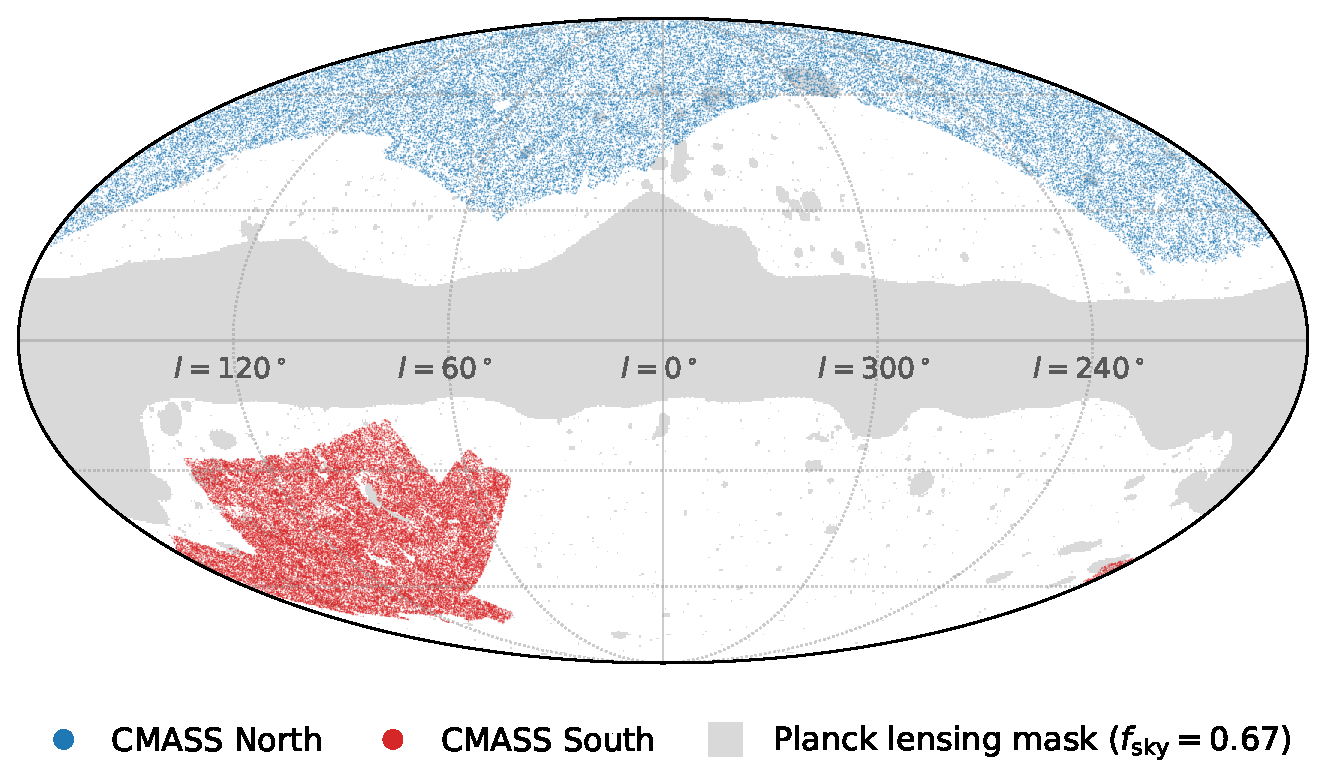
\includegraphics[width=0.48\linewidth]{footprint.pdf}
  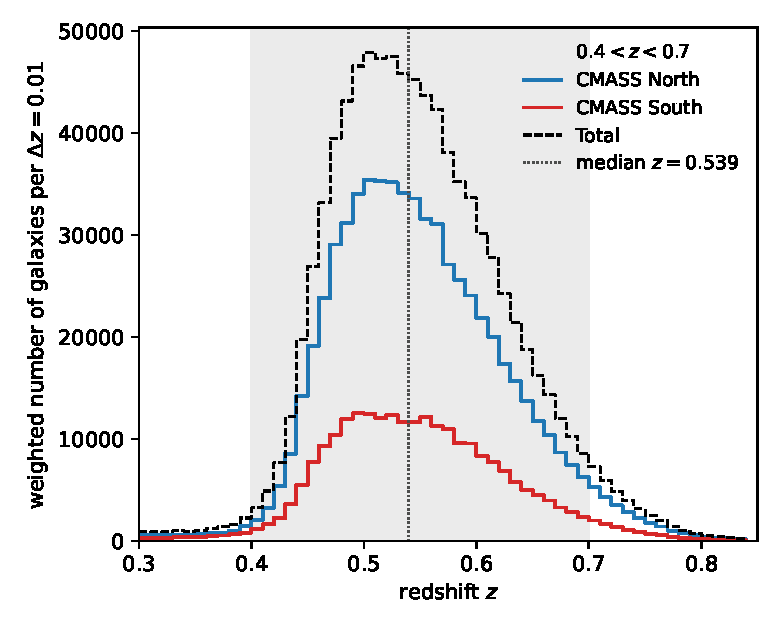
\includegraphics[width=0.48\linewidth]{zdist.pdf}
  \caption{Left: footprint of the BOSS CMASS North and South samples in
  Galactic coordinates, overlaid on the Planck 2018 lensing analysis mask.
  Right: weighted redshift distribution of the CMASS galaxies in each cap
  and in total, with the $0.4<z<0.7$ selection shaded and the median
  redshift of the selected sample marked.
  }
  \label{fig:footprint_zdist}
\end{figure}

\subsection{Random catalogs}
\label{sec:data_random}

The BOSS random catalogs \citep{Reid2016} sample the angular selection
function of each cap at roughly fifty times the galaxy density, with
redshifts assigned from the observed galaxy distribution. The randoms
therefore share the galaxies' $n(z)$ but contain no clustering. We apply the
same $0.4<z<0.7$ cut and use the full catalogs, $40.9$ million points over
both caps, for every random stack. Replacing the full catalog by a 10 percent
subsample shifts the $10\,\hinvMpc$ bridge excess by
$5\times10^{-4}$, comparable to the measured signal.
% CHECK: combine_filament_jackknife.py docstring.
Random points carry unit systematic weight and, in the single-galaxy stacks,
the same lensing-efficiency weight as the galaxies.

The randoms serve three purposes. First, a stack of the convergence map
around random points measures the mean convergence of the footprint,
including any residual mean-field or mask-related offset, and is subtracted
from the single-galaxy stack. Second, pairs of random points selected with
the same separation criteria as the galaxy pairs provide the equivalent
correction for the pair stack. Because the number of random pairs is of
order $10^{9}$, the full random catalog is needed to reduce the noise in this
correction. Third, a seeded 10 percent subsample of the randoms traces the
survey footprint on a coarse HEALPix grid to define the jackknife regions
used for error estimation (Section~\ref{sec:method}).

\subsection{Planck CMB lensing map}
\label{sec:data_planck}

We use the Planck 2018 lensing reconstruction \citep{Planck2018lensing},
release \texttt{COM\_Lensing\_4096\_R3.00}. The convergence harmonic
coefficients $\kappa_{LM}$ are taken from the minimum-variance combination
of the temperature and polarization quadratic estimators applied to the
SMICA foreground-cleaned maps. The Planck pipeline subtracts the estimator
mean field, and the coefficients are provided up to
$L_{\rm max}=4096$. As discussed in Section~\ref{sec:intro}, the
reconstruction is noise dominated on the small angular scales relevant to
this work.

Before stacking we multiply $\kappa_{LM}$ by a Gaussian beam of
$8\,\mathrm{arcmin}$ full width at half maximum and synthesize a HEALPix map
\citep{Gorski2005} at $N_{\rm side}=2048$, corresponding to a pixel scale of
$1.7\,\mathrm{arcmin}$. This smoothing suppresses small-scale reconstruction
noise. At $z=0.55$, $8\,\mathrm{arcmin}$ spans
$\simeq3.3\,\hinvMpc$ comoving. We test the dependence on smoothing scale in
Section~\ref{sec:method}. We sample the smoothed map at the sky positions
corresponding to the comoving stack grid by nearest-pixel lookup, without
interpolation.

We apply the Planck lensing analysis mask distributed with the release,
which removes the Galactic plane, point sources, and regions of poor
foreground cleaning and retains 67.1 percent of the sky. Masked pixels
receive zero weight in every stack, so that the stacked value at each grid
position is a weighted mean over unmasked pixels only. The CMASS footprint
lies almost entirely within the unmasked region: 96.5 percent of North and
94.7 percent of South galaxies, 96.0 percent overall, fall on unmasked
pixels. The remainder lie mostly in the point-source and cluster holes of the
mask and at the low-latitude edge of the North cap
(Fig.~\ref{fig:footprint_zdist}).
% CHECK: the fraction whose full 100 h^-1 Mpc cutout is unmasked is not yet computed.

\subsection{$N$-body simulation and mock catalog}
\label{sec:sim}

We calculate the $\Lambda$CDM reference signal from the BigMDPL run of the
MultiDark suite \citep{Klypin2016, Riebe2013}, a dark-matter-only simulation
of a periodic box $2500\,\hinvMpc$ on a side with $3840^{3}$ particles of mass
$2.36\times10^{10}\,h^{-1}\mathrm{M}_{\odot}$ in a Planck cosmology with
$\Omega_{\rm m}=0.307$ and $h=0.678$. We use the snapshot at $a=0.6464$,
$z=0.547$, close to the weighted mean redshift of the CMASS sample. Haloes
are taken from the public Rockstar catalog; we keep host haloes only,
discarding subhaloes, and use the Rockstar virial mass $M_{\rm vir}$. The
HOD is applied to hosts with
$\log_{10}(M_{\rm vir}/h^{-1}\mathrm{M}_{\odot})\geq12.5$.

Mock galaxies are placed with a central-only halo occupation distribution of
the form adopted for CMASS by \citet{White2011},
\begin{equation}
  \langle N_{\rm cen}\rangle(M) = \tfrac{1}{2}\left[1+\mathrm{erf}
  \left(\frac{\ln(M/M_{\rm cut})}{\sqrt{2}\,\sigma}\right)\right],
  \label{eq:hod}
\end{equation}
with $\sigma=0.94$ in $\ln M$. We use
$\log_{10}(M_{\rm cut}/h^{-1}\mathrm{M}_{\odot})=13.246$, rather than the
value $13.04$ adopted by \citet{White2011}. With our halo definition and
catalog mass floor, the latter gives a number density of
$4.21\times10^{-4}\,h^{3}\,\mathrm{Mpc}^{-3}$. We set the threshold to match
the CMASS central-galaxy density,
$2.70\times10^{-4}\,h^{3}\,\mathrm{Mpc}^{-3}$: the observed density of
$3\times10^{-4}\,h^{3}\,\mathrm{Mpc}^{-3}$ multiplied by a central fraction
of 0.9.
% Provenance: analysis/sim/results/galaxies_hod_nmatch.csv.meta.json
% (run 2026-07-20, occupation seed 20260720). 13.246 solves nbar = 0.9 * 3e-4
% over hosts_minmass12p5.bin; make_hod_catalog.py still defaults to the
% published White+11 value 13.04, so the paper run passes --log10-mcut.
Each host receives a galaxy with probability $\langle N_{\rm cen}\rangle$.
The input halo catalog ends at the stated mass floor, where the adopted
occupation is still $0.034$, and therefore truncates the low-mass tail of
the model. The mock contains no satellites, whereas about 10 percent of
CMASS galaxies are satellites \citep{White2011}; we return to this limitation
in Section~\ref{sec:discussion}. Halo peculiar velocities are included in
the redshift-space pair selection.

The second halo sample used for the sensitivity tests consists of hosts
within $\pm0.05$ dex of
$\log_{10}(M_{\rm vir}/h^{-1}\mathrm{M}_{\odot})=13.0$
(Section~\ref{sec:method}).

The simulated convergence map is built from the public 1-in-200 particle
subsample, which contains $2.8\times10^{8}$ particles. Each sampled particle
has an effective mass equal to 200 simulation particles. We project the
particles along one box axis through
the full $2500\,\hinvMpc$ depth onto a periodic grid of $0.1\,\hinvMpc$
pixels. If $N_{\rm p}(\boldsymbol{x})$ is the number of particles in a pixel
of width $\ell$, $N_{\rm tot}$ is the total number of projected particles,
and $L$ is the box width, the mean-subtracted surface density is
$\Sigma(\boldsymbol{x})=m_{\rm eff}[N_{\rm p}(\boldsymbol{x})/\ell^{2}
-N_{\rm tot}/L^{2}]$. We convert it to convergence as
$\kappa=\Sigma/\Sigma_{\rm crit}$ with the comoving critical density for a
lens at $z=0.547$ and the CMB as source,
$\Sigma_{\rm crit}=8.88\times10^{14}\,h\,\mathrm{M}_{\odot}\,{\rm Mpc}^{-2}$.
The map is smoothed with a periodic two-dimensional Gaussian of FWHM
$3.31\,\hinvMpc$, which is $8\,\mathrm{arcmin}$ at the comoving distance
$1424.5\,\hinvMpc$ of the snapshot. Because the box is projected at a single
redshift, the mock reproduces the mean signal of structure correlated with
the pairs but not the full line-of-sight integral or the Planck
reconstruction noise; it is used for the reference signal, not for the
observational covariance. The single-galaxy stack from this map has been
checked against an independent direct particle-count estimator; the two
agree to 3 percent inside $10\,\hinvMpc$.

Mock pairs are selected in redshift space from a random 50 percent subsample
of the catalog, which reduces the pair count while preserving the halo-mass
selection in expectation. The projection axis serves as the line of sight,
and each galaxy's coordinate along it is displaced by
$(1+z)\,v_{\parallel}/H(z)$, where $v_{\parallel}$ is its line-of-sight
peculiar velocity, before the line-of-sight cut is applied. This models the
effect of peculiar velocities on the pair selection. Transverse
separations are computed with periodic boundaries.
Nonphysical pairs, close in projection but separated along the line of
sight in real space by $20$--$120\,\hinvMpc$, are selected from the same
catalog. They are not close in three dimensions and therefore provide a null
test of the control.

% ---------------------------------------------------------------------------
% Methods + Results draft -- consolidated from the former "Theoretical
% Expectation" and "Measurement Results" sections.
%
% Written against the checked-in pipeline documented in paper/README.md:
%   lib/geometry.py (two_halo_template, band_profile, kappa_band),
%   lib/jackknife.py, stack_single_jk.py, stack_pairs_jk.py,
%   find_and_stack_pairs.py, combine_jackknife.py,
%   combine_filament_jackknife.py, fit_band_covariance.py,
%   fit_sim_template.py, analysis/sim/*.
%
% Conventions:
%   % CHECK  -- a number recorded in the repo (notes, docstrings, figures)
%               but not reproducible from checked-in result files.
%   % TODO   -- a quantity the pipeline produces but whose value is not in
%               the repo at all; fill from the run outputs / Google Doc.
%   % UNVERIFIED -- describes code or results that are not yet supported by
%               checked-in outputs.
%
% Structure: \section{Methods}, \section{Expected signal from the simulation},
% \section{Results}.
%
% ---------------------------------------------------------------------------

\section{Methods}
\label{sec:method}

The data and mock use the same pair selection, pair-frame stacking, halo
control, and band statistic. The observed stacks also include survey weights,
the Planck mask, and random-catalog subtraction. The mock map is periodic and
has zero mean, so the mock stacks are unweighted and require no random-catalog
subtraction. Observed errors use a spatial jackknife over the footprint; mock
errors use blocks of the simulation box.

\subsection{Pair selection}
\label{sec:pairs}

For every galaxy we compute the comoving distance $D_{\rm c}=\chi(z)\,h$ from
its spectroscopic redshift. Two galaxies form a pair if their line-of-sight
and transverse separations,
\begin{equation}
  r_{\parallel} = |D_{{\rm c},1}-D_{{\rm c},2}|, \qquad
  r_{\perp} = \theta_{12}\,\frac{D_{{\rm c},1}+D_{{\rm c},2}}{2},
  \label{eq:separations}
\end{equation}
with $\theta_{12}$ the great-circle angle between them, satisfy
$r_{\parallel}\leq r_{\parallel,{\rm max}}$ and
$r_{\perp,{\rm min}}\leq r_{\perp}\leq r_{\perp,{\rm max}}$. Because
$r_{\parallel}$ is computed from redshifts it is a redshift-space quantity
and includes the pairwise peculiar velocity (Section~\ref{sec:intro}). We
use three transverse bins, $4$--$6$, $9$--$11$, and $18$--$22\,\hinvMpc$,
referred to below as the $5$, $10$, and $20\,\hinvMpc$ samples, with
line-of-sight cuts of $r_{\parallel,{\rm max}}=5\,\hinvMpc$ for the
$5\,\hinvMpc$ sample and $10\,\hinvMpc$ for the other two. The cuts were
fixed on the mock before the observed stacks were examined
(Section~\ref{sec:sim_expect}). Each unordered pair is counted once. A
galaxy may belong to several pairs and we apply no isolation criterion; the
resulting correlation between pairs is handled by the spatial jackknife
rather than by down-weighting. The pair is assigned the comoving distance
$D_{\rm mid}=\chi(\bar z)\,h$ at the mean redshift of its members. Random
pairs are selected from the full random catalogs with the same criteria.

\subsection{Stacking in the pair frame}
\label{sec:stacking}

Each pair defines a local Cartesian frame on the sky: the $X$ axis runs
from galaxy 1 to galaxy 2, with the pair ordered so that $X$ increases with
Galactic longitude, and the $Y$ axis is perpendicular to it. Galaxy 1 and
galaxy 2 sit at $X=\mp r_{\perp}/2$, $Y=0$, at their own separation, so
within a bin the halo positions spread over the bin width. We lay down a
$101\times101$ grid of points spanning $\pm50\,\hinvMpc$ in both
directions, a spacing of exactly $1\,\hinvMpc$ with a grid point at the
midpoint. A grid point $(X,Y)$ is mapped to Galactic coordinates in the
small-angle approximation,
\begin{equation}
  \Delta l\cos b_{\rm c} = \frac{X\cos\phi - Y\sin\phi}{D_{\rm mid}}, \qquad
  \Delta b = \frac{X\sin\phi + Y\cos\phi}{D_{\rm mid}},
  \label{eq:grid_to_sky}
\end{equation}
where $(l_{\rm c},b_{\rm c})$ is the pair midpoint and $\phi$ is the
position angle of the pair axis, defined by
$(\cos\phi,\sin\phi)\propto(\Delta l\cos b_{\rm c},\Delta b)$.
Each sky position is assigned the value of the HEALPix pixel that contains
it. At $N_{\rm side}=2048$ the pixel scale of $1.7\,\mathrm{arcmin}$ is
finer than the grid spacing, which is $2.4\,\mathrm{arcmin}$ at $z=0.55$,
so no interpolation is applied. Masked pixels receive zero weight. The rare
pairs whose grid extends past a Galactic pole are dropped.

The stacked map is the weighted mean at each grid point,
\begin{equation}
  \hat\kappa(X,Y) = \frac{\sum_{i} w_{i}\,m_{i}(X,Y)\,\kappa_{i}(X,Y)}
                         {\sum_{i} w_{i}\,m_{i}(X,Y)},
  \label{eq:stack}
\end{equation}
where $i$ runs over pairs, $w_{i}=w_{1}w_{2}$ is the pair weight
(Section~\ref{sec:data_cmass}), and $m_{i}\in\{0,1\}$ is the mask value at
the sampled pixel. The pair frame has a four-fold symmetry: the two
galaxies are statistically interchangeable, and the sky above and below the
axis is equivalent. We therefore replace the value at $(X,Y)$ by the mean of
the four symmetry-related pixels $(\pm X,\pm Y)$, removing residual
asymmetries between the two members and across the pair axis.

Single galaxies and single random points are stacked in the same way on a
$100\times100$ grid of $1\,\hinvMpc$ cells centered on the object, with the
axes aligned with Galactic longitude and latitude and the weight $w$ of
Equation~(\ref{eq:weights}) multiplied by the lensing-efficiency factor
(Section~\ref{sec:data_cmass}). Because a single stack has no preferred
direction it is symmetrized radially: pixels are averaged in annuli about
the physical center of the grid, which for an even grid lies between the
four central pixels.

\subsection{Joint footprint and random subtraction}
\label{sec:joint}

The North and South caps form a single weighted sample in
Equation~(\ref{eq:stack}). This differs from averaging two per-cap maps:
with $73$ percent of the galaxies in the North, an equal-weight average
would give each Southern galaxy $2.7$ times the influence of a Northern one
and would carry the noisier Southern map into the combined profile at half
weight.
Single galaxies and single randoms are stacked by the same code with the
same weights, and the corrected single map is their difference,
$\hat\kappa_{\rm g}-\hat\kappa_{\rm r}$. The random-point map absorbs the
mean convergence of the footprint and any offset associated with the mask
or the mean field of the reconstruction.

Random pairs are stacked separately for each cap and combined with weights
proportional to the number of pairs in each. The random-pair map is
subtracted from the galaxy-pair map and held fixed in the error analysis.
Its bridge statistic has magnitude at most $4.1\times10^{-5}$ across the
three samples, compared with observed jackknife errors of at least
$2.2\times10^{-4}$.

\subsection{Control for the halo contributions}
\label{sec:control}

The pair stack contains the one-halo and isotropic two-halo contributions of
both members in addition to any anisotropic excess (Section~\ref{sec:intro}).
We model the isotropic part with a control built from the corrected single
stack. Let $P(r)$ be the radial profile of the radially symmetrized
corrected single map, interpolated linearly in radius. The control for a
pair of separation $d$ is the superposition
\begin{equation}
  T(X,Y) = P\!\left(\sqrt{(X-d/2)^{2}+Y^{2}}\right)
         + P\!\left(\sqrt{(X+d/2)^{2}+Y^{2}}\right),
  \label{eq:control}
\end{equation}
evaluated at the bin-center separation on the $101\times101$ pair grid. It
has unit amplitude and no free parameters. We define the residual map as
\begin{equation}
  F(X,Y) = \left[\hat\kappa_{\rm gp}(X,Y)-\hat\kappa_{\rm rp}(X,Y)\right]
           - T(X,Y),
  \label{eq:filament}
\end{equation}
where gp and rp denote the galaxy-pair and random-pair stacks.

The control represents two average CMASS galaxies placed at the pair
positions and subtracts their measured mean isotropic signal. It does not
remove differences between the environments of paired and average galaxies.
Such differences remain in $F$ as residual convergence around the galaxies
and as structure aligned with the pair axis. The single stack includes the
lensing-efficiency weight, whereas the pair stack does not; the control and
pair map therefore have different redshift weights, and the analysis does
not correct this mismatch. The mock is processed with the same control and
band statistic (Section~\ref{sec:sim_expect}). We do not fit the amplitude of
$T$ to the pair stack because fitting axis-aligned structure would allow the
control to absorb the bridge signal. Section~\ref{sec:robust} tests this
effect on the mock.

\subsection{Band statistic}
\label{sec:bands}

Rather than interpret the two-dimensional map pixel by pixel, we compress
$F$ into a profile along the pair axis. For each column $X$ we take the
mean of $F$ in a central band $|Y|\leq1.5\,\hinvMpc$, where a filament
would lie, and in an off-center band $1.5\leq|Y|\leq10.5\,\hinvMpc$ that
brackets it, and form their difference,
\begin{equation}
  B(X) = \langle F(X,Y)\rangle_{|Y|\leq1.5}
       - \langle F(X,Y)\rangle_{1.5\leq|Y|\leq10.5}.
  \label{eq:band}
\end{equation}
The band widths are fixed in comoving units at every separation, so all
three samples use the same physical bands. Rows straddling a band
boundary are given fractional weights equal to the fraction of the row that
lies inside the band, so the statistic does not depend on where pixel edges
fall; on the $101$ grid the bands are three and eighteen whole rows. The
difference suppresses components that vary slowly with $Y$ and removes an
offset shared by both bands. It reduces the map to one number per position
along the axis. The bridge excess is the mean of $B(X)$ over the
window $|X|\leq0.35\,d$ between the galaxies, which stops $0.15\,d$ short of
each halo center. For covariance-based fits the profile is further compressed
into a vector of the central and off-center band means in eleven bins of
$4\,\hinvMpc$ along $X\geq0$, $22$ numbers in all. The first ten bins span
$0\leq X<40\,\hinvMpc$, and the endpoint at $X=40\,\hinvMpc$ forms the
eleventh bin. The binning reduces the dimension of the covariance while
retaining resolution comparable to the smoothing scale.

The $3.3\,\hinvMpc$ smoothing scale moves part of any narrow bridge signal
into the off-center band. Equation~(\ref{eq:band}) is therefore a filtered
observable rather than an estimate of the unsmoothed peak convergence. We
apply the same filtering to the data and mock. The ratio of the bridge
statistic to the central-band excess in the mock provides a transfer factor
between these two quantities.
% TODO: quote the transfer factor (bridge excess / central-band excess) from the mock.

\subsection{Errors and covariance}
\label{sec:errors}

Errors on the observed maps come from a delete-one spatial jackknife. We
partition the joint footprint into $K=287$ contiguous,
approximately equal-occupancy regions based on HEALPix cells with
$N_{\rm side}=10$, with an RMS size scatter of $11$ percent.
% CHECK: 287 and 11% are quoted in CLAUDE.md and code docstrings; the regions file is not in the repo.
No region straddles the two caps. Galaxies and random points are assigned to
regions by their positions and pairs by their midpoints. Galaxies and randoms
use the same regions, so each realization applies the same spatial deletion
to every term in the corrected map. For any statistic $x$ (a pixel, a band
value, or the compressed vector), the jackknife variance and covariance are
\begin{equation}
  \sigma^{2}=\frac{K-1}{K}\sum_{k=1}^{K}(x_{k}-\bar x)^{2}, \qquad
  \mathsf{C}=\frac{K-1}{K}\sum_{k=1}^{K}(\mathbf{x}_{k}-\bar{\mathbf{x}})
                                          (\mathbf{x}_{k}-\bar{\mathbf{x}})^{\mathsf T},
  \label{eq:jackknife}
\end{equation}
with $\bar x$ the mean of the leave-one-out values. The full chain of
Equations~(\ref{eq:control})--(\ref{eq:band}) is rebuilt inside every
realization: the control is regenerated from the leave-one-out single stack
and subtracted from the leave-one-out pair stack, so the uncertainty of the
control propagates into the bridge error. The random-pair map is the one
quantity held fixed.

The covariance matters because the $8$-arcmin smoothing scale spans more than
three grid pixels. Treating pixels or $1\,\hinvMpc$ bins as independent
understates the error on a band mean by a factor of $2.2$ to $2.6$ on the
joint stack. % CHECK: CLAUDE.md and fit_sim_template.py docstring.
All quoted errors on band quantities are jackknife errors on the quantity
itself, and all fits use $\mathsf{C}$. For $K=287$ and a $22$-element vector,
the nominal Hartlap factor is $0.920$. Applying it to $\mathsf{C}^{-1}$ would
increase the fitted amplitude errors by $4.3$ percent. We do not apply it
because the leave-one-out jackknife samples are correlated rather than
independent covariance realizations.

Where we fit the amplitude $A$ of a fixed template $\mathbf{s}$ to an
observed vector $\mathbf{d}$ we use
\begin{equation}
  \begin{aligned}
  \chi^{2}(A) &=(\mathbf{d}-A\mathbf{s})^{\mathsf T}\mathsf{C}^{-1}
                 (\mathbf{d}-A\mathbf{s}), \\
  \hat A &=\frac{\mathbf{s}^{\mathsf T}\mathsf{C}^{-1}\mathbf{d}}
                 {\mathbf{s}^{\mathsf T}\mathsf{C}^{-1}\mathbf{s}}, \qquad
  \sigma_{A}=\left(\mathbf{s}^{\mathsf T}\mathsf{C}^{-1}\mathbf{s}\right)^{-1/2}.
  \end{aligned}
  \label{eq:amplitude}
\end{equation}
We test for an additive constant by nesting a model with a free offset.

\subsection{The simulated pipeline}
\label{sec:sim_pipeline}

The mock analysis repeats Sections~\ref{sec:stacking}--\ref{sec:bands} on
the simulated convergence map of Section~\ref{sec:sim}. Mock pairs are
selected in redshift space with the same $r_{\perp}$ bins and
$r_{\parallel}$ cuts as the data.
Mock pairs and mock single galaxies are unweighted. The single stack uses
every mock galaxy, so the control uses the same superposed-single construction
as the data. The periodic zero-mean map requires no random-pair subtraction.
Errors come from a delete-one jackknife over a $5\times5$ tiling of the box
face, with $500\,\hinvMpc$ blocks assigned by pair midpoint and the same
$(K-1)/K$ estimator. The control is held fixed in the mock jackknife, so the
mock errors include block-to-block variation of the pair stack but not
sampling uncertainty in the single stack.

Three further mock products are used. First, a line-of-sight sweep repeats
the pair selection with $r_{\parallel,{\rm max}}=5$, $10$, $20$, and
$30\,\hinvMpc$ and records, for each cut, the completeness (the fraction of
truly associated pairs, real-space $|r_{\parallel}|\leq20\,\hinvMpc$, that
survive the redshift-space cut), the interloper fraction (the fraction of
selected pairs whose real-space separation exceeds $20\,\hinvMpc$), and a
bridge-sensitivity metric. The production cuts were fixed before the
observed stacks were examined.
% CHECK: state the cut-selection rule after reconciling los_contamination_table.py and rpar_scan.py.
Second, a non-physical-pair test stacks mock pairs with real-space
line-of-sight separations of $20$--$40$, $40$--$60$, $60$--$90$, and
$90$--$120\,\hinvMpc$ and checks whether the control leaves a residual bridge.
Third, a sensitivity grid varies the smoothing, the $r_{\parallel}$ cut, the
bin half-width, and the halo mass of the tracer sample.

\section{Expected signal from the simulation}
\label{sec:sim_expect}

Figure~\ref{fig:sim_pair_vs_control} shows the mock pair stack at
$r_{\perp}=10\,\hinvMpc$ beside its control. On a common color scale the
two are nearly indistinguishable because the residual is small compared with
the signal around the galaxies. Subtracting the control leaves the pattern
shown in Figure~\ref{fig:sim_residual_maps} at all three separations: a positive
ridge along the pair axis between the galaxies and a deficit above and
below it. In the mock, the matter distribution around selected pairs is
anisotropic; subtracting an isotropic control leaves positive residuals along
the pair axis and negative residuals perpendicular to it. The band difference
of Equation~(\ref{eq:band}) measures this contrast.

\begin{figure*}
  \centering
  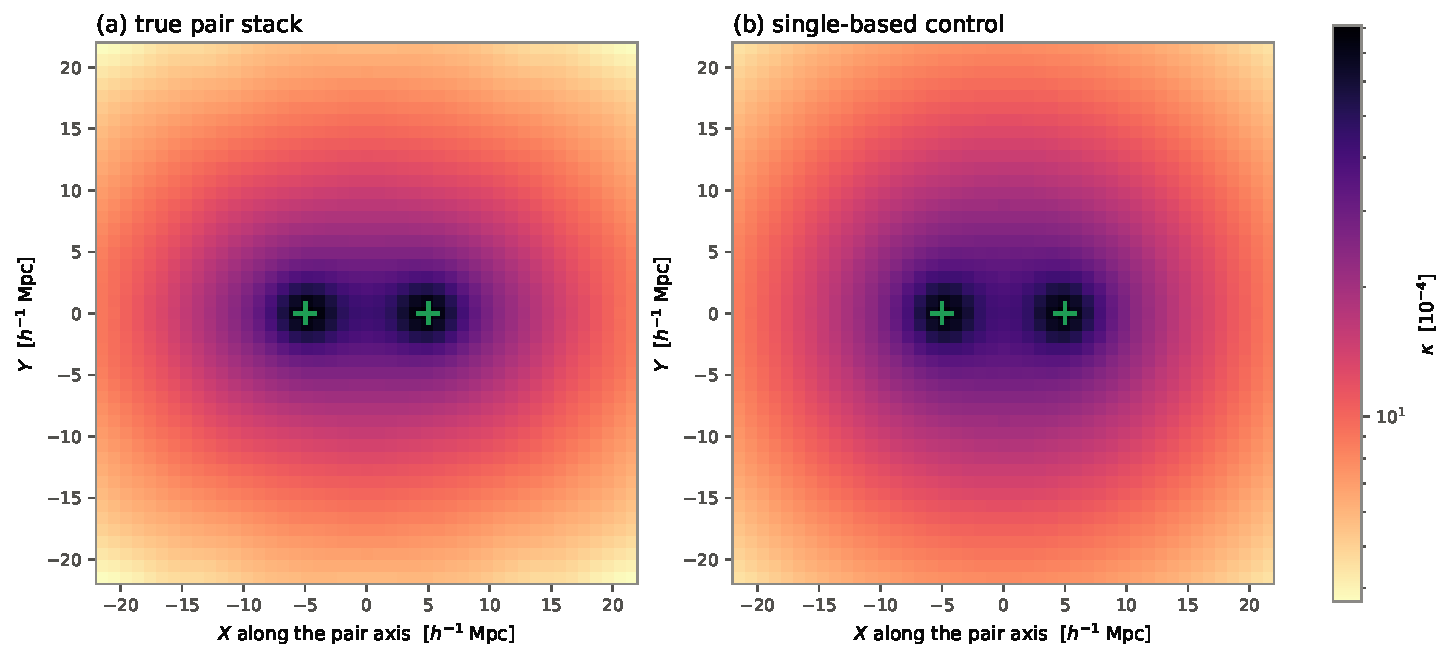
\includegraphics[width=0.9\linewidth]{Figure/sim_pair_vs_control_maps_sep10.pdf}
  \caption{Mock pair stack at $r_{\perp}=10\,\hinvMpc$ (left) and its
  unit-amplitude control, Equation~(\ref{eq:control}) (right), on a common
  color scale.}
  \label{fig:sim_pair_vs_control}
\end{figure*}

\begin{figure*}
  \centering
  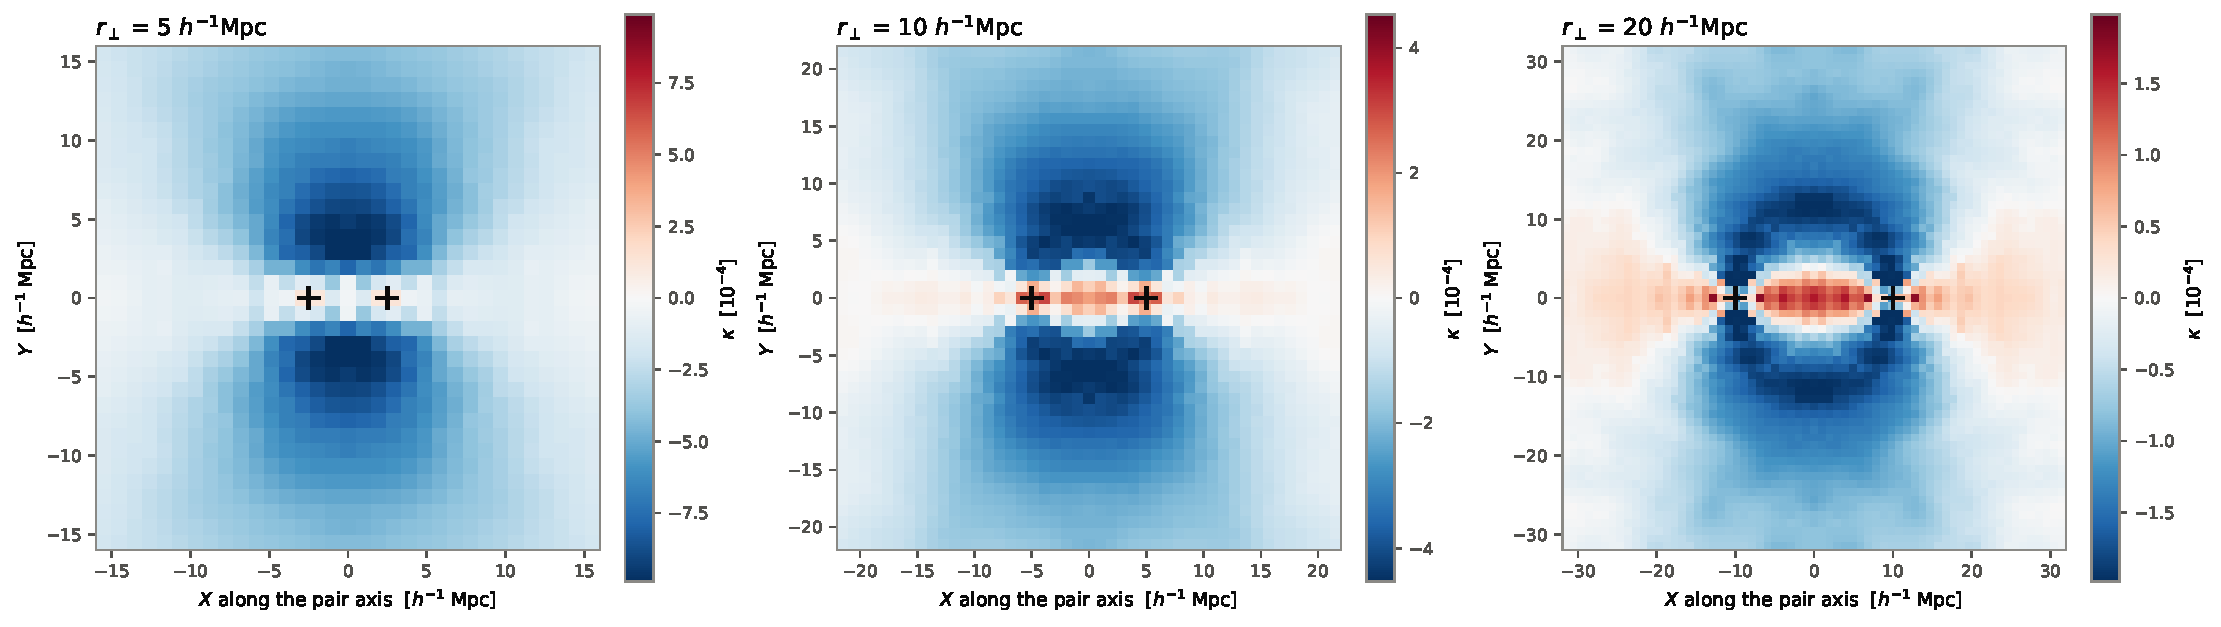
\includegraphics[width=0.9\linewidth]{Figure/sim_quadrupole_diff_maps.pdf}
  \caption{Mock residual maps $F$ at $r_{\perp}=5$, $10$, and $20\,\hinvMpc$
  (left to right), showing the ridge along the pair axis and the deficit
  perpendicular to it. Galaxy positions are marked.}
  \label{fig:sim_residual_maps}
\end{figure*}

Figure~\ref{fig:sim_band_profiles} shows the band profiles. The bridge
excess in the mock is
$\left(6.32\pm0.36,\ 4.91\pm0.21,\ 2.18\pm0.12\right)\times10^{-4}$ at
$r_{\perp}=5$, $10$, and $20\,\hinvMpc$. The corresponding $25$-block
jackknife signal-to-noise ratios are $17.7$, $22.9$, and $18.1$.
The decrease is consistent with a lower connected-pair fraction and lower
mean bridge density at larger separation. The mock residual also contains an
approximately isotropic component at the galaxy positions and an anisotropic
component along the pair axis.
% TODO: quote the mock residual at the halo positions and the midpoint kappa.

\begin{figure*}
  \centering
  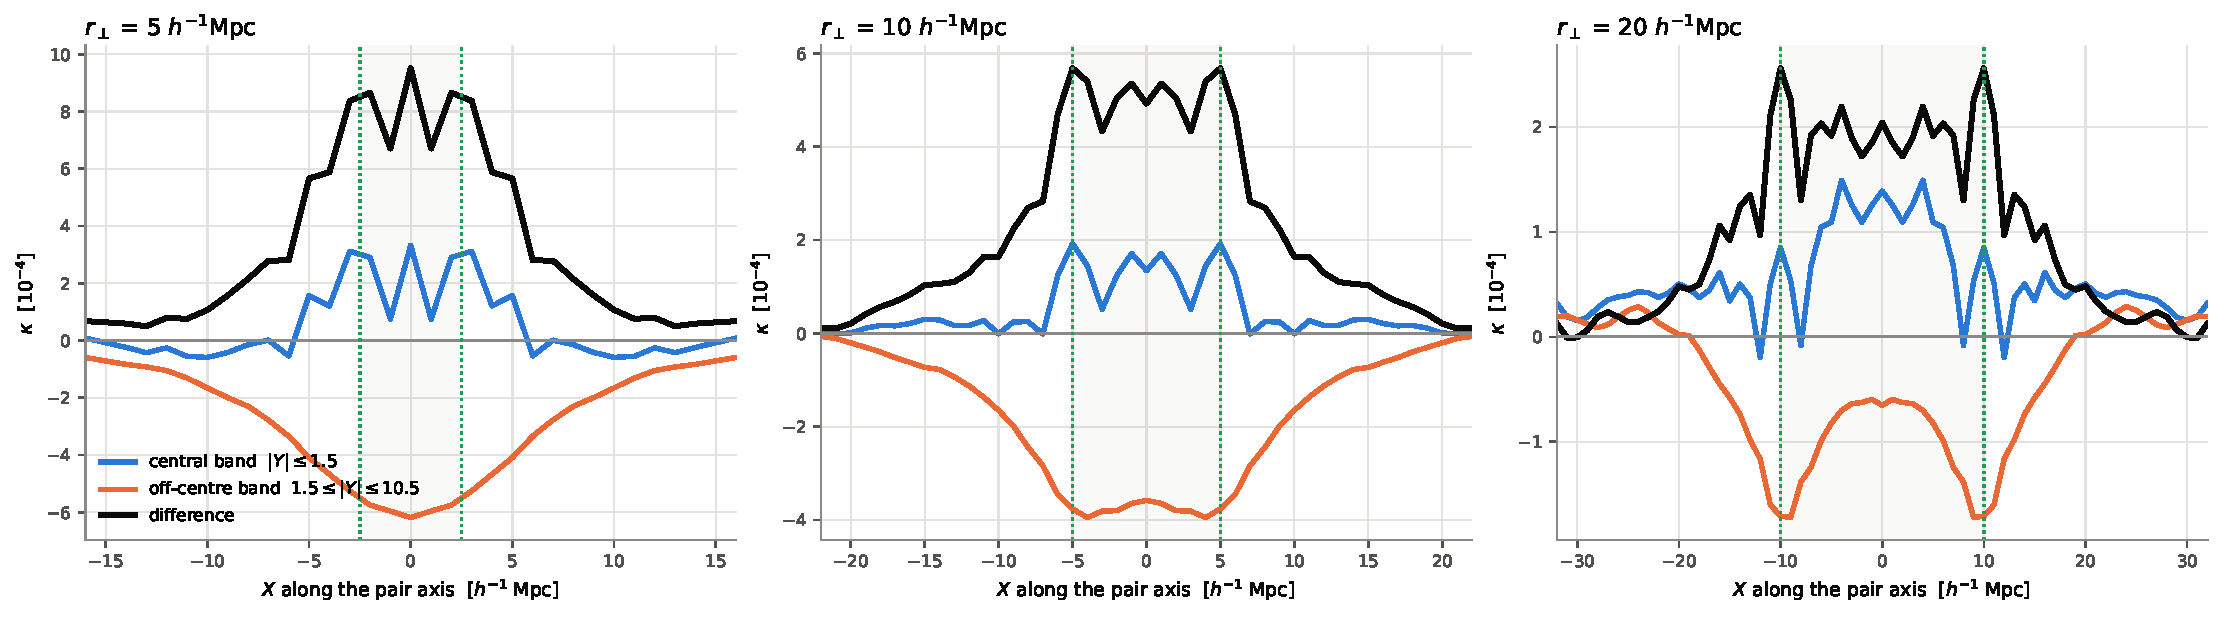
\includegraphics[width=0.9\linewidth]{Figure/sim_band_profiles_all_seps.pdf}
  \caption{Central-band mean, off-center-band mean, and their difference
  $B(X)$ for the mock residual maps at the three separations. The shaded
  window is $|X|\leq0.35\,d$.}
  \label{fig:sim_band_profiles}
\end{figure*}

The non-physical mock pairs show no bridge in any line-of-sight band,
confirming that the control does not itself generate a ridge.
% TODO: per-band residual bridge excess +/- error from nonphysical_pair_test_*.csv.
The line-of-sight sweep motivates the production cuts: at
$r_{\perp}=5\,\hinvMpc$ the bridge signal first rises and then falls as the
cut is widened, while at $10\,\hinvMpc$ it falls.
% TODO: completeness / interloper fraction / sensitivity per cut from rpar_scan.csv and los_sweep_summary.csv.

\section{Results}
\label{sec:results}

\subsection{Observed stacks}
\label{sec:obs_stacks}

The three BOSS samples contain $217{,}702$, $459{,}051$, and
$1{,}282{,}969$ pairs at $r_{\perp}=5$, $10$, and $20\,\hinvMpc$.
Figure~\ref{fig:boss_maps} shows the corrected single stack and the three
corrected pair stacks. Figure~\ref{fig:obs_vs_sim_maps} compares the
observed residual maps with the simulated ones. The observed maps contain a
broad axis-aligned excess and off-axis deficit, but these features have low
signal-to-noise in the Planck reconstruction.

\begin{figure*}
  \centering
  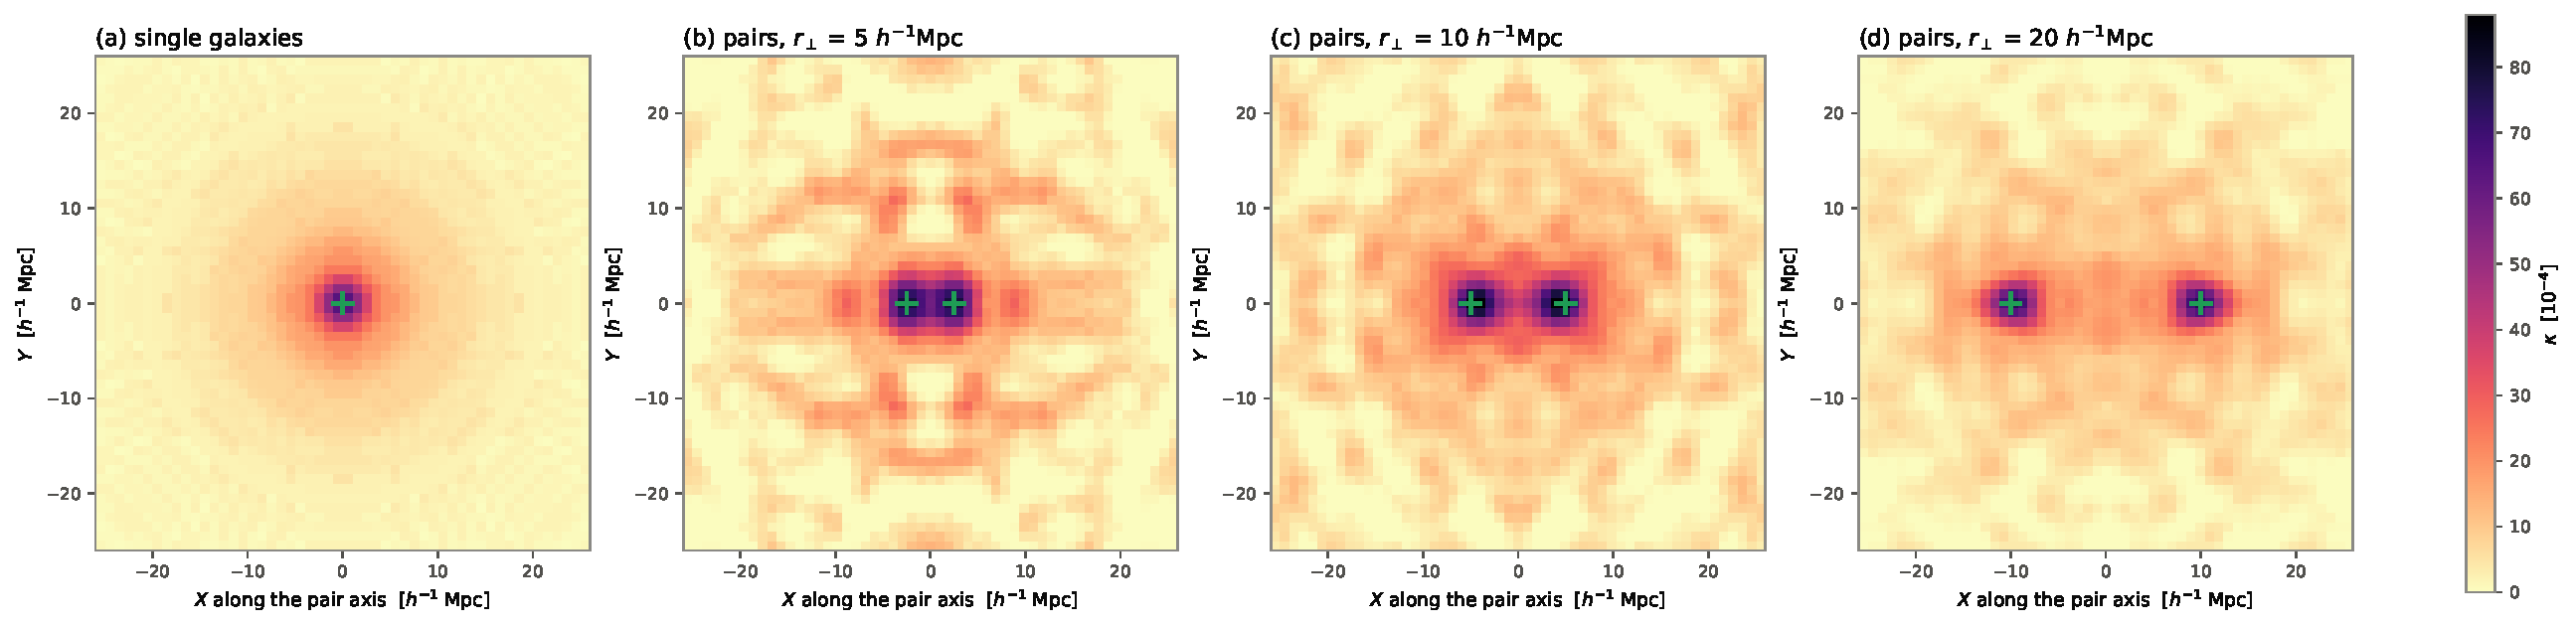
\includegraphics[width=0.9\linewidth]{Figure/boss_single_and_pair_maps.pdf}
  \caption{Corrected BOSS single-galaxy stack (left) and corrected pair
  stacks at $r_{\perp}=5$, $10$, and $20\,\hinvMpc$.}
  \label{fig:boss_maps}
\end{figure*}

\begin{figure*}
  \centering
  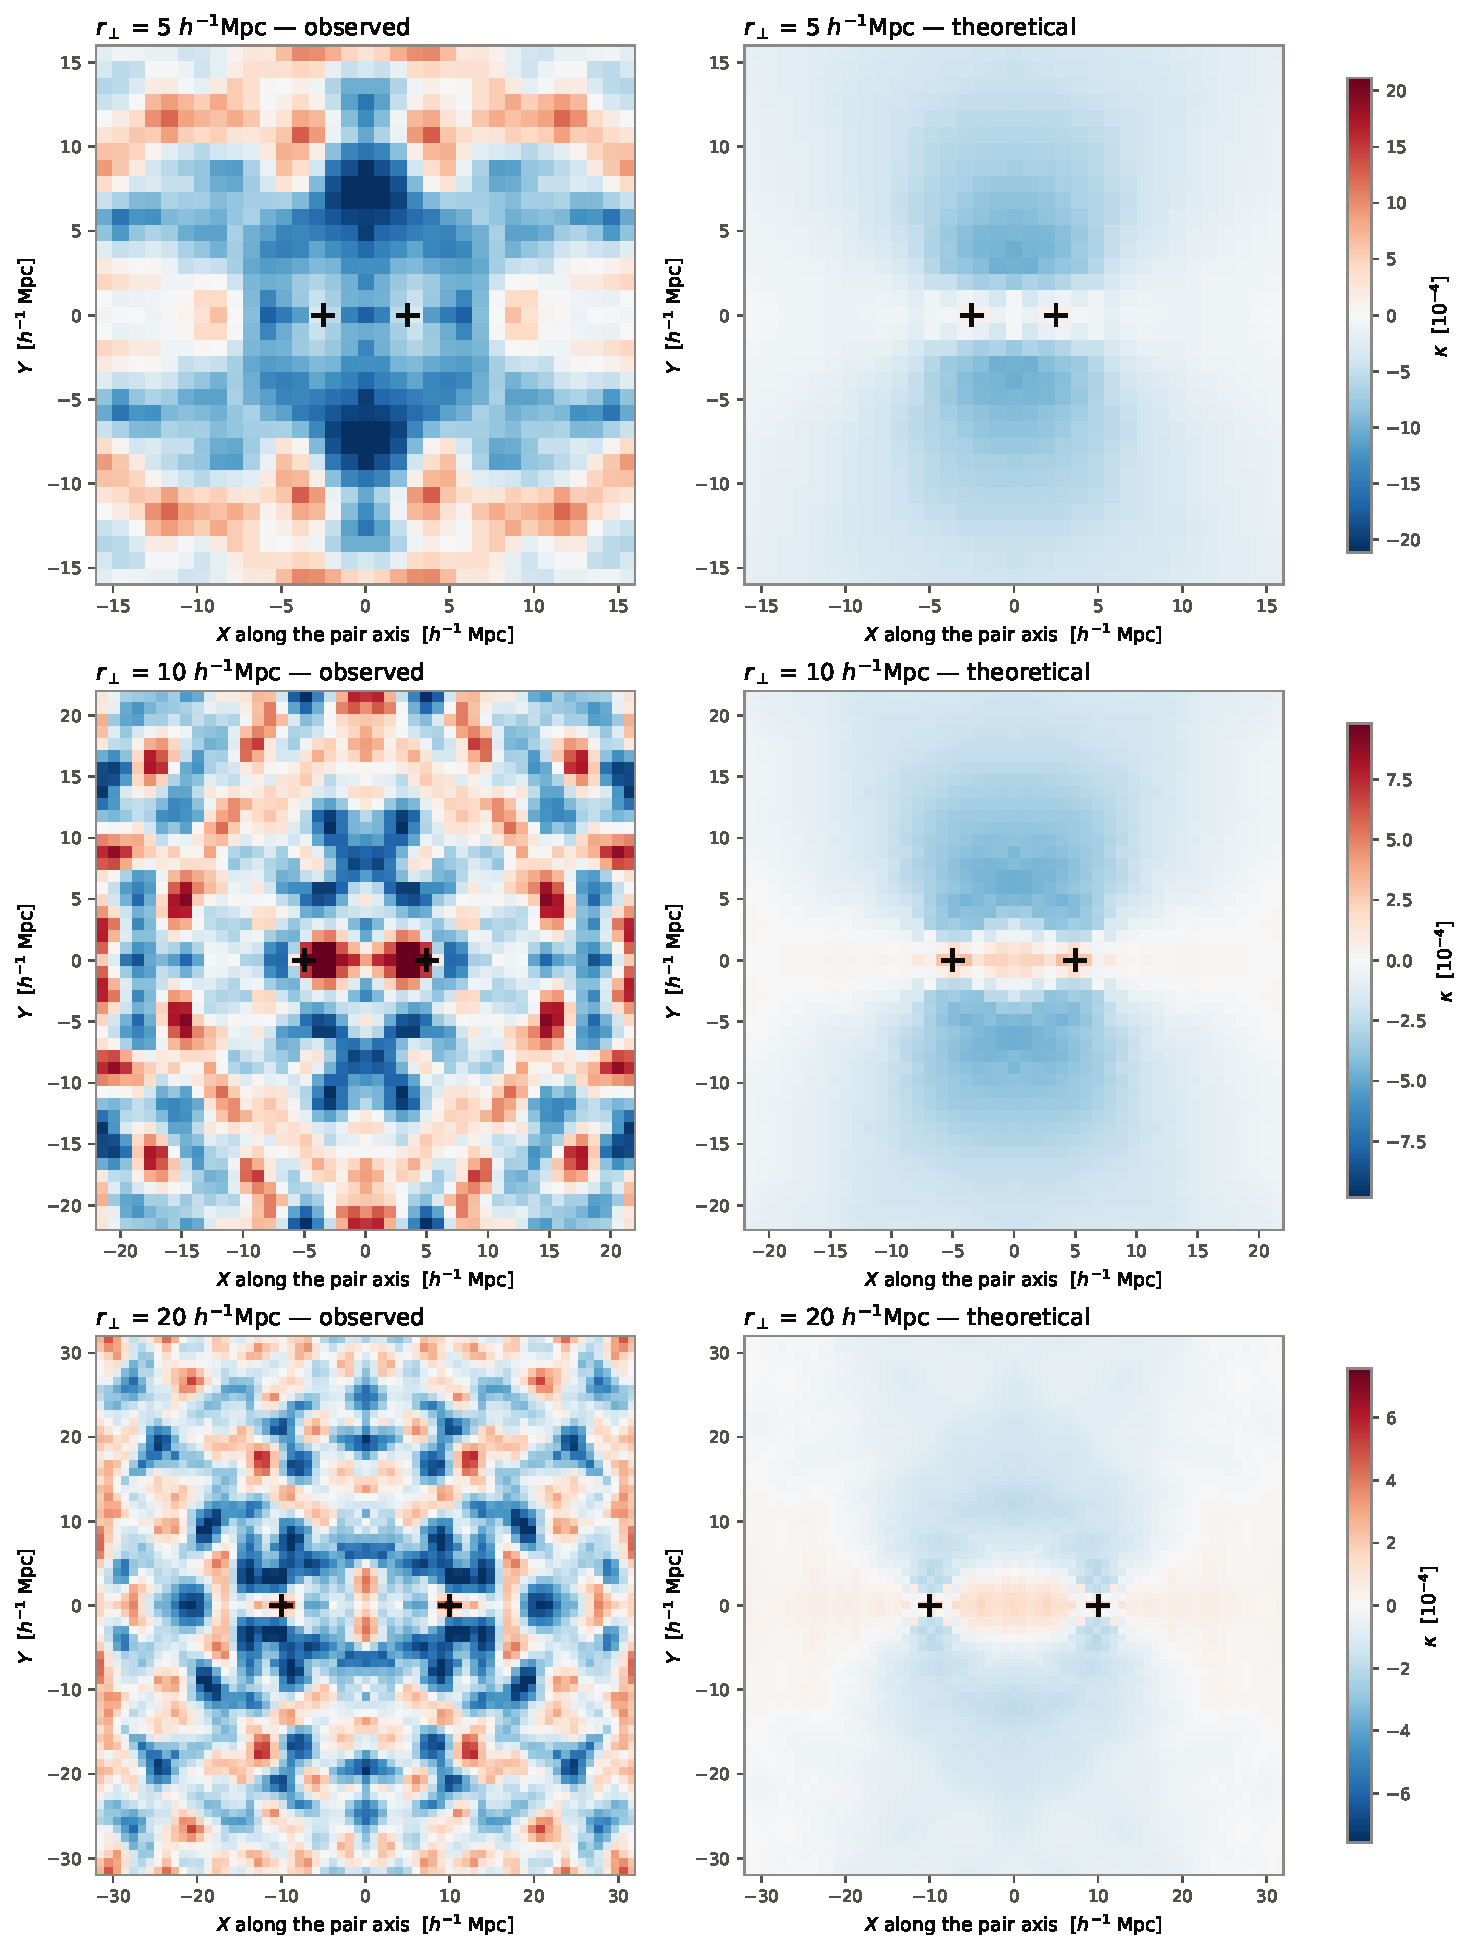
\includegraphics[width=0.7\linewidth]{Figure/obs_vs_sim_quadrupole_maps.pdf}
  \caption{Observed (left) and simulated (right) residual maps at
  $r_{\perp}=5$, $10$, and $20\,\hinvMpc$ (top to bottom), on a common
  color scale per row.}
  \label{fig:obs_vs_sim_maps}
\end{figure*}

\subsection{Bridge convergence}
\label{sec:bridge}

Table~\ref{tab:bridge} lists the bridge excess in each sample with its
jackknife error, beside the mock prediction in the same statistic.
Figure~\ref{fig:band_profiles_obs_sim} overlays the observed band profiles
on the mock prediction.

\begin{table}
  \centering
  \caption{Bridge excess, Equation~(\ref{eq:band}) averaged over
  $|X|\leq0.35\,d$, for the three BOSS samples, with the mock prediction in
  the same statistic. Observed errors are from the $287$-region delete-one
  jackknife with the control rebuilt in every realization; mock errors from
  the $25$-block jackknife. The final column is the observed-minus-mock
  difference divided by the quadrature sum of their errors.}
  \label{tab:bridge}
  \begin{tabular}{cccccc}
    \hline
    $r_{\perp}$ & $N_{\rm pairs}$ & Observed & S/N & Mock & Obs.$-$Mock \\
    $[\hinvMpc]$ & & $[10^{-4}]$ & & $[10^{-4}]$ & $[\sigma]$ \\
    \hline
    5  & $217{,}702$   & $5.38\pm9.08$  & $0.6$ & $6.32\pm0.36$ & $-0.1$ \\
    10 & $459{,}051$   & $11.91\pm5.10$ & $2.3$ & $4.91\pm0.21$ & $+1.4$ \\
    20 & $1{,}282{,}969$ & $1.24\pm2.22$  & $0.6$ & $2.18\pm0.12$ & $-0.4$ \\
    \hline
  \end{tabular}
\end{table}

\begin{figure*}
  \centering
  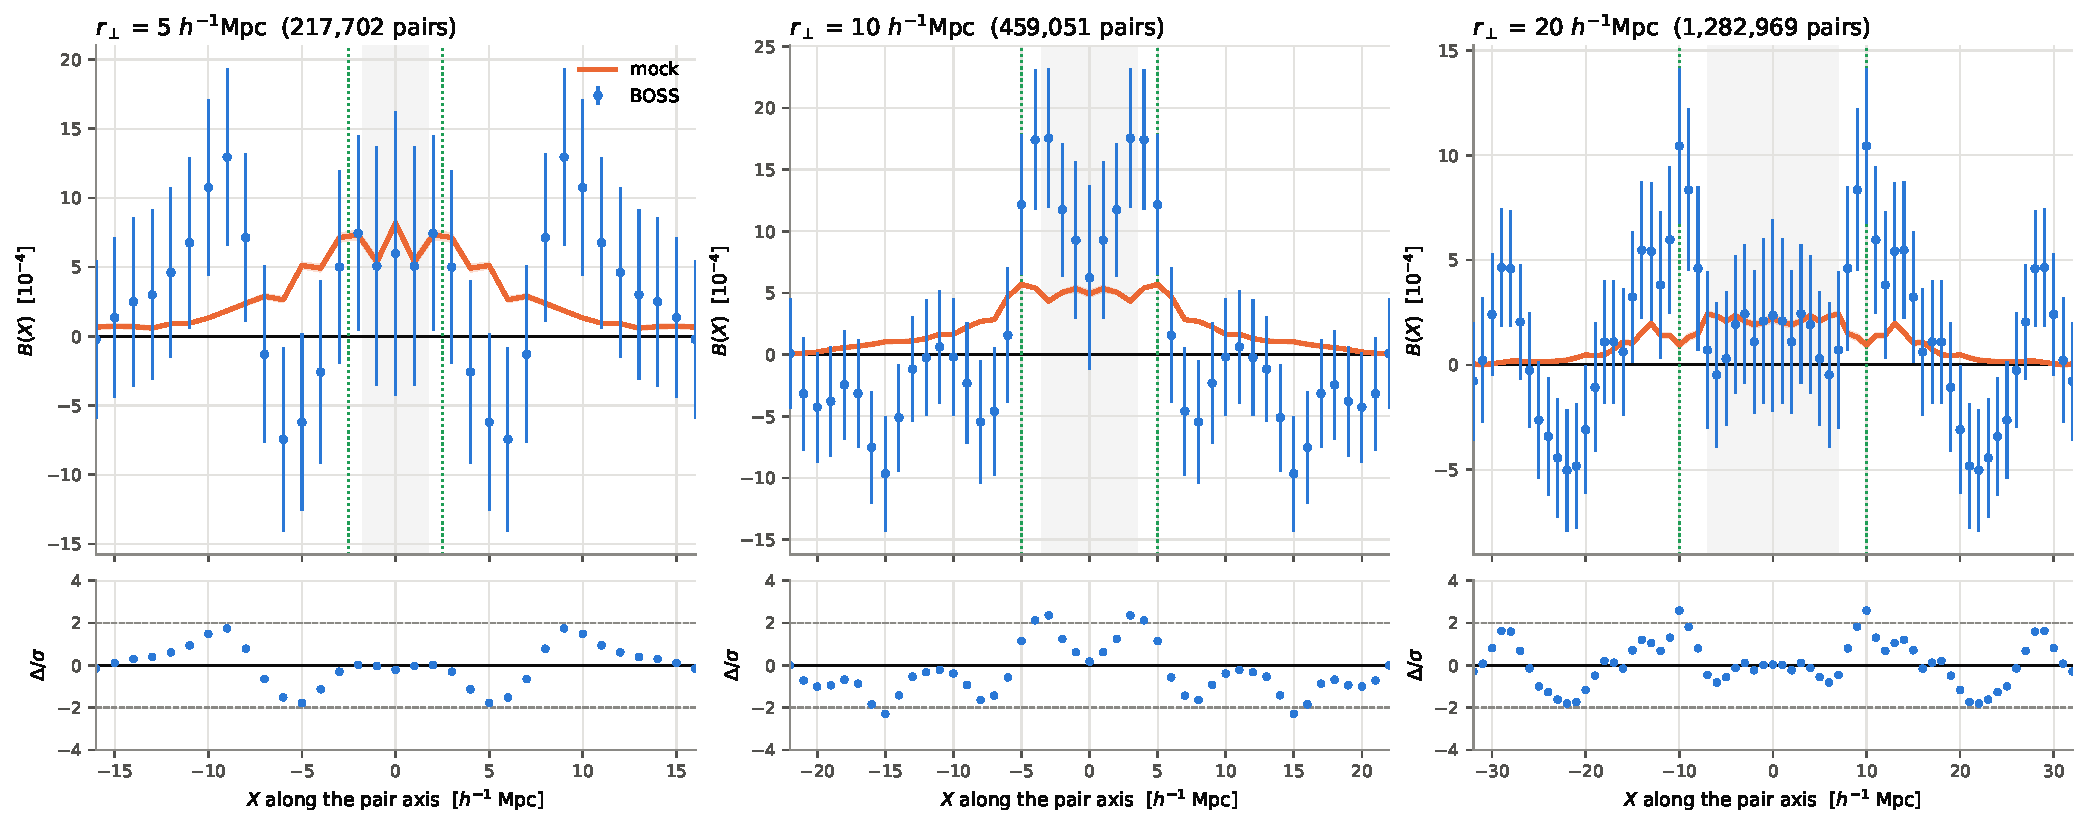
\includegraphics[width=0.9\linewidth]{Figure/band_profiles_obs_vs_sim.pdf}
  \caption{Observed band profile $B(X)$ with jackknife errors (points) and
  the mock prediction with its box-jackknife band (shaded) at the three
  separations. The observed errors are delete-one jackknife over the
  $287$ sky patches; the mock band is the $25$-block box jackknife, with
  the superposed-singles control held fixed across realizations. Gray marks
  the bridge window $|X| \leq 0.35\,d$; dotted green lines mark the galaxy
  positions.
  Lower panels: difference in units of the observed error, with dashed
  guides at $\pm2$. The mock pairs are selected in the same
  transverse bins as BOSS at all three separations. The mock band is
  statistical only: it is the $25$-block scatter of a single realization and
  excludes the uncertainty in the HOD.}
  \label{fig:band_profiles_obs_sim}
\end{figure*}

No bridge excess exceeds $3\sigma$. The $10\,\hinvMpc$ sample has a positive
excess of $2.3\sigma$ and lies $1.4\sigma$ above the mock prediction; the
other two bridge excesses are consistent with zero.
A $\chi^{2}$ test of the compressed $22$-element profile against zero with
the full covariance gives $\chi^{2}=35.0$, $20.7$, and $32.4$ for $22$
degrees of freedom (nominal $p=0.04$, $0.54$, and $0.07$). The $p=0.04$
result at $5\,\hinvMpc$ is a full-profile departure from zero, not a bridge detection:
the test includes the bins containing the galaxies.

Fitting the amplitude of the mock residual profile to the observed profile with
Equation~(\ref{eq:amplitude}) over the full $22$-element vector returns
$A=1.47\pm0.36$, $1.07\pm0.49$, and $1.60\pm0.57$, at $4.1$, $2.2$, and
$2.8\sigma$.
At $10$ and $20\,\hinvMpc$, bins around the galaxies contribute $59$ and
$44$ percent of the fitted response. At $5\,\hinvMpc$, the
$4\,\hinvMpc$ binning places the galaxy positions in the only bridge bin,
so their contributions cannot be separated. The full-profile amplitude
is therefore not a bridge amplitude. Restricting the fit to the bridge window
$|X|\leq0.35\,d$ gives $A=1.97\pm0.58$, $1.81\pm0.84$, and $0.71\pm0.95$, at
$3.4$, $2.1$, and $0.7\sigma$. These significances differ from the bridge
excesses in Table~\ref{tab:bridge} because the fit treats the central and
off-center bands as separate data elements, whereas the bridge statistic
uses their difference. The $5\,\hinvMpc$ fit still contains the unresolved
galaxy bin, and beam-convolved halo signal can enter the bridge window at all
three separations. We therefore use these fits as profile diagnostics rather
than bridge detections. A nested test that adds a free constant to the full
profile leaves the amplitudes unchanged and returns offsets of
$\left(-1.6,\ +0.4,\ +0.2\right)\times10^{-4}$, consistent with zero.

\subsection{Comparison with the simulation and with previous work}
\label{sec:compare}

The direct data--mock comparison is the bridge statistic in
Table~\ref{tab:bridge}, for which both maps use the same bands, bridge window,
and smoothing. The observed uncertainties exceed the predicted bridge
amplitudes at all three separations, and the measurements are consistent with
both zero and the mock.

A $95$ percent upper limit on the bridge excess can be converted to a surface
density using $\Sigma_{\rm crit}$ and then to a linear mass density over the
bridge length.
% TODO: compute the upper limits and compare them with Epps & Hudson (2017) and de Graaff et al. (2019).

The residual maps also test whether the control describes the paired haloes.
The observed residual map peaks at the galaxy positions at about
$2\times10^{-3}$, compared with $0.9\times10^{-3}$ in the mock.
% CHECK: values from the fit_sim_template.py docstring; confirm from checked-in output.
If confirmed, this difference means that paired CMASS galaxies have a larger
excess over the average CMASS galaxy than paired mock galaxies have over the
average mock galaxy. A central-only HOD with a soft mass threshold may produce
a different pair selection from the observed sample, which includes
satellites and a stellar-mass selection. The corrected single-galaxy profile
also lies below the matched mock prediction at large radius.
% CHECK: fit_sim_template.py docstring; compare_boss_mock_profile.py retracted earlier significance values.
These comparisons constrain the isotropic residual from which the
axis-aligned signal is separated; they do not directly measure the bridge
statistic because Equation~(\ref{eq:band}) subtracts the off-center band.
% TODO: compare corrected single profiles in the 10--20, 15--25, and 20--40 h^-1 Mpc bands with jackknife errors.

\citet{deGraaff2019} measured
$\bar\kappa=(5.8\pm3.1)\times10^{-4}$ in the bridge region of pairs pooled
over $6$--$14\,\hinvMpc$. Their statistic differs from ours in four ways:
pairs are rescaled to unit separation before stacking, the bridge region is
defined on the rescaled grid, the halo model is fitted to the pair stack in
a $60^\circ$ sector about the direction perpendicular to the pair axis, and
the map is smoothed to $10$ arcmin. Their central value is numerically close
to our $10\,\hinvMpc$ result, but the two estimators are not identical. Their
sample contains about $2.2$ times as many pairs as our $10\,\hinvMpc$
sample; independent-pair scaling alone would reduce the error by a factor of
$1.5$.
Pooling our three samples with inverse-variance weights would provide an
approximate comparison, but it would remain a different estimator from that
of \citet{deGraaff2019}.
% TODO: quote the pooled value if this comparison is retained.

\subsection{Robustness tests}
\label{sec:robust}

\paragraph{Smoothing.} Figure~\ref{fig:smoothing_scan} compares the observed
$8$- and $6$-arcmin results at all three separations and the $4$-arcmin
result at $5$ and $10\,\hinvMpc$. The bridge signal-to-noise values for
$8$, $6$, and $4$ arcmin are $(0.6,1.2,2.2)$ at $5\,\hinvMpc$ and
$(2.3,2.4,1.1)$ at $10\,\hinvMpc$; at $20\,\hinvMpc$ the $8$- and
$6$-arcmin values are $0.6$ and $0.5$. We retain $8$ arcmin as the common
smoothing scale and do not tune it separately for each separation.

\begin{figure}
  \centering
  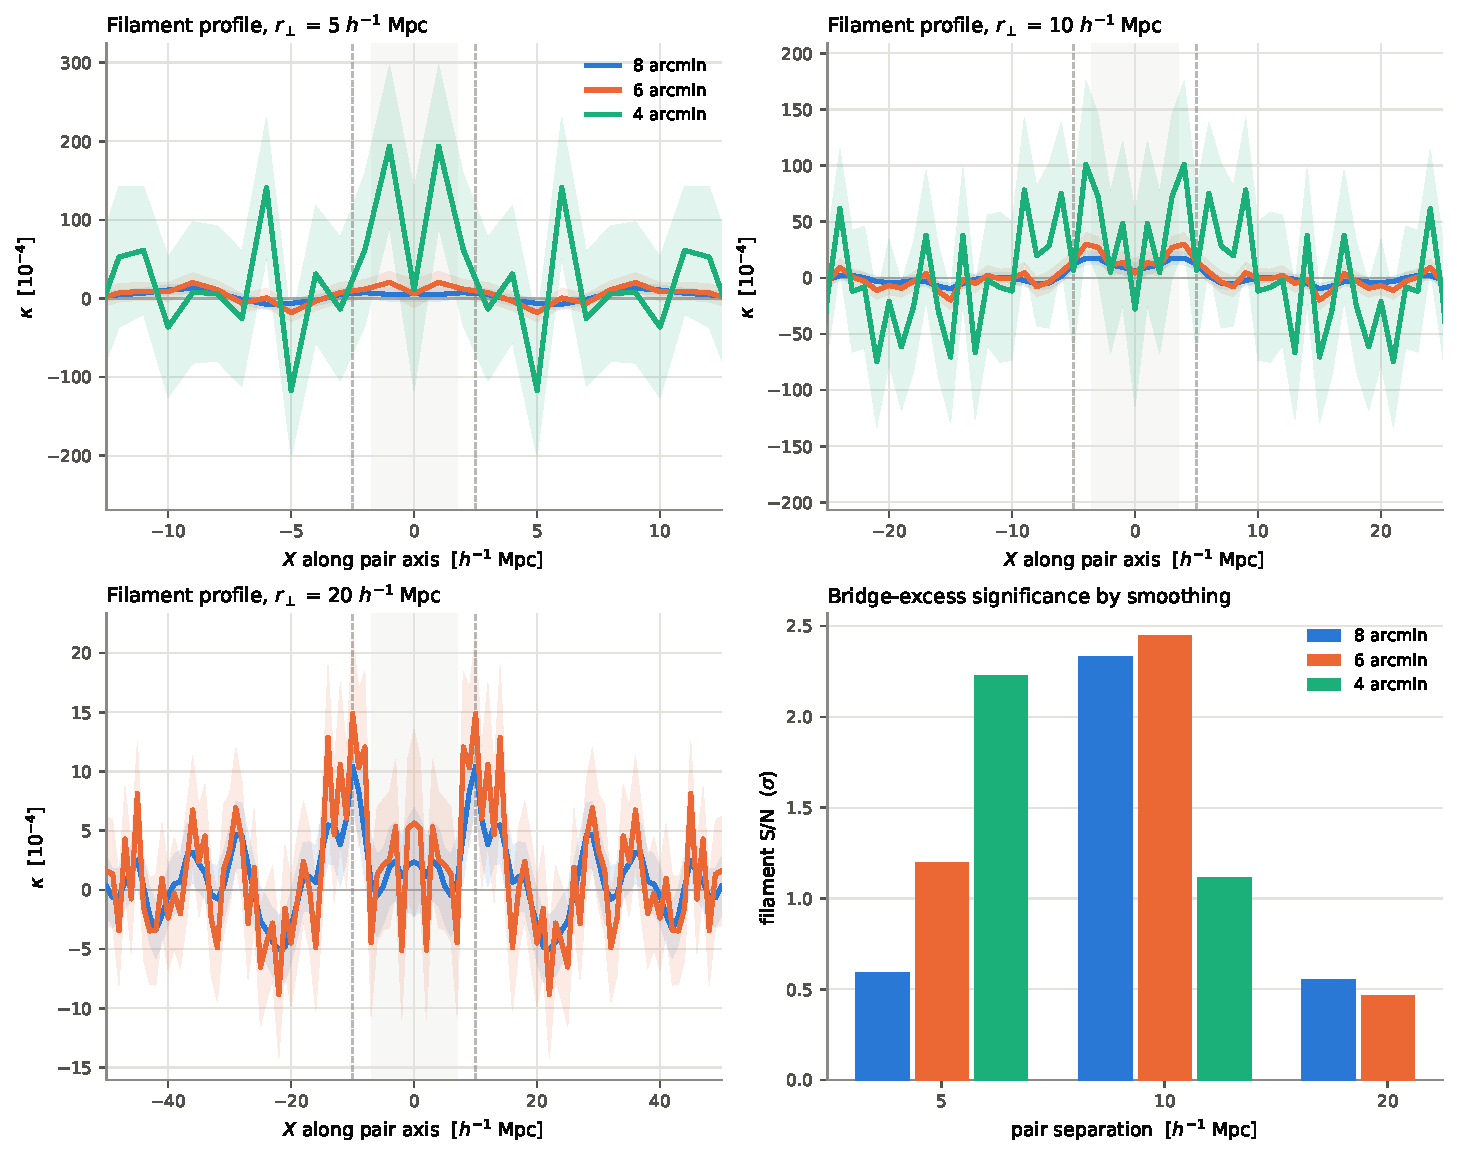
\includegraphics[width=\linewidth]{Figure/filament_snr_vs_smoothing.pdf}
  \caption{Observed bridge profiles and signal-to-noise for the available
  smoothing FWHM values. The $4$-arcmin stack is unavailable at
  $20\,\hinvMpc$.}
  \label{fig:smoothing_scan}
\end{figure}

\paragraph{Weighting.} The effect of removing the lensing-efficiency weight
from the single stacks has not yet been quantified.
% TODO: report the changes in the control and bridge excess.
Combining the two caps by an equal-weight average instead of the joint stack
produced the apparent dip reported in earlier versions of this analysis.
% TODO: report the shift in the corrected single profile at 20 h^-1 Mpc.

\paragraph{Random-pair sample.} Replacing the full random catalog by a
10 percent subsample shifts the $10\,\hinvMpc$ bridge excess by
$5\times10^{-4}$, comparable to the signal, which is why the full randoms
are required. % CHECK: combine_filament_jackknife.py docstring.

\paragraph{Fitted control.}
% UNVERIFIED: align this description with band_core_tail_control.py and add checked-in results.
As an alternative to the unit-amplitude control, we split the single-galaxy
profile into core and tail components and fit their amplitudes outside the
pair. On the mock this control drives the bridge excess to zero at all three
separations, whereas the unfitted control recovers the known bridge. The
fitted control therefore absorbs axis-aligned signal, and we do not use it
for the headline measurement.
% TODO: quote mock and observed bridge excess under the fitted control beside the unfitted values.

% ---------------------------------------------------------------------------
% Summary and Discussion draft -- written to close the argument opened in
% notes/intro_draft.tex and carried through notes/methods_results_draft.tex.
% Same conventions: % CHECK / % TODO / % UNVERIFIED (see methods draft header).
%
% Each bold lead below answers one of the four "differences from de Graaff"
% promised in the introduction, in the same order, then discusses what the
% mock comparison taught us and what comes next.
% ---------------------------------------------------------------------------

\section{Summary and Discussion}
\label{sec:discussion}

We have stacked the Planck 2018 lensing convergence map on $217{,}702$,
$459{,}051$, and $1{,}282{,}969$ BOSS CMASS galaxy pairs at transverse
separations of $5$, $10$, and $20\,\hinvMpc$,
subtracted a control built from the galaxies' own single-galaxy stack, and
measured the convergence left between the pair members. The same pipeline
was run on a CMASS-like mock built from the BigMDPL simulation, which
supplies the $\Lambda$CDM expectation for every quantity we measure.

\textbf{We do not detect a filament, and the data cannot yet test the
$\Lambda$CDM prediction.} The bridge excess is consistent with zero at all
three separations, at $0.6\sigma$, $2.3\sigma$, and $0.6\sigma$.
Testing the compressed profile against zero with the full covariance gives
the same conclusion. The mock predicts a bridge of $6.32\pm0.36$,
$4.91\pm0.21$, and $2.18\pm0.12\times10^{-4}$ in the same statistic,
at or below our errors at every separation --- comfortably so at
$5\,\hinvMpc$, but by only a few per cent at $10$ and $20\,\hinvMpc$ --- so
the observations cannot distinguish the prediction from no bridge at all.
At $10\,\hinvMpc$ the measurement sits $2.3\sigma$ from zero and $1.4\sigma$
from the mock, so such preference as there is runs mildly towards the
prediction rather than away from it.
% TODO: 95 per cent upper limits as Sigma and linear mass density.
The $2.3\sigma$ excess at $10\,\hinvMpc$ is at the level of the
$1.9\sigma$ signal that \citet{deGraaff2019} found in the same data with a
different estimator, and we regard the two as the same marginal hint.

\textbf{Resolving the measurement in separation costs sensitivity that
Planck cannot afford.} The first change we made relative to
\citet{deGraaff2019} was to bin pairs by separation on a fixed comoving grid
rather than rescaling and pooling them. The mock shows why this is worth
doing: the predicted bridge falls by a factor of three from $5$ to
$20\,\hinvMpc$, so the pooled measurement mixes structures of very
different amplitude. But dividing the sample raises the error in each bin,
and at Planck noise none of the bins is individually informative. Pooling
our three bins with inverse-variance weights gives
$3.05\pm1.99\times10^{-4}$, or $1.5\sigma$, which is the number to compare
with theirs. The three samples are drawn from one catalogue over one
footprint and share galaxies, so this error, which assumes they are
independent, is a lower bound.

\textbf{The limit is the map, not the method.} Removing the control
entirely and measuring the same window on the raw band changes the error
only marginally,
% TODO: quote the exact change from the committed pipeline (the 7 per cent figure came from the fitted-control analysis).
so the error budget is set by the Planck reconstruction noise within the
bridge window and not by the uncertainty of the control. No refinement of
the template can shrink the error bar; only more pairs or a less noisy
convergence map can. Treating pixels as independent would have understated
the error by a factor of $2.2$ to $2.6$, % CHECK
which is the single largest source of over-optimism in a measurement of
this kind.

\textbf{The unit-amplitude control is the right choice, and the mock says
why.} The third change was to use a control with no fitted parameters. On
the mock, the unit-amplitude control recovers a clear bridge with the
expected decline in separation, whereas a control whose core and tail
amplitudes are fitted to the region outside the pair drives the residual to
zero at every separation. % UNVERIFIED: fitted-control code not in the repo
The pair axis is aligned with the surrounding large-scale structure on both
sides of the pair, so any region along the axis is correlated with the
bridge and a fit there absorbs it. This is the weakness of profile fitting
that we anticipated in Section~\ref{sec:intro}, now measured on a
simulation with known content. The non-physical mock pairs, with
line-of-sight separations of $20$--$120\,\hinvMpc$, show no bridge with the
unit-amplitude control, % TODO: values
so the control does not manufacture a ridge on its own.

\textbf{The control is not perfect, and the imperfection is informative.}
The observed filament map retains a residual of about $2\times10^{-3}$ at
the galaxy positions against $0.9\times10^{-3}$ in the mock. % CHECK
Galaxies with a close companion live in more massive haloes than the
average CMASS galaxy, and this selection is stronger in the data than in a
central-only mock with a soft mass threshold. Independently, the BOSS
single-galaxy profile falls below the mock at large radius. % CHECK
Both discrepancies affect the isotropic residual, which the band difference
removes to first order, but they set the size of the halo signal that leaks
toward the bridge window, and they mean the mock does not reproduce the
data's leakage exactly. Two improvements to the mock follow directly. The
HOD should include satellites, which contribute the close pairs at
$5\,\hinvMpc$ and raise the mass selection in pairs, and it should be tuned
on the measured single-galaxy lensing profile rather than on the number
density alone.

\textbf{The bridge window must clear the beam.} The window
$|X|\leq0.35\,d$ ends $0.15\,d$ from each halo centre: $0.75\,\hinvMpc$ at
$d=5$, $1.5$ at $d=10$, and $3\,\hinvMpc$ at $d=20$, against a smoothed halo
profile of $3.3\,\hinvMpc$ at half maximum. Because the central band at a
given $X$ lies closer to the halo than the off-centre band, an isotropic
halo residual leaks into the band difference with a positive sign. In an
earlier version of this analysis, excluding only $\pm1\,\hinvMpc$ around
each halo produced an apparent $2.4\sigma$ bridge that vanished once the
exclusion reached a full beam width. % CHECK: from the earlier (uncommitted) analysis; confirm the numbers or drop the sentence
At $5\,\hinvMpc$ a beam-wide exclusion leaves no window at all, which is
why we treat that bin as a consistency check on the two larger ones rather
than as an independent measurement, and why the $5\,\hinvMpc$ mock bridge
should be read as bridge plus halo leakage. % TODO: quote the mock leakage estimate (B(X) with the filament removed, or with randomised pair orientations)
The general lesson is that any pair-stacking bridge statistic needs an
exclusion of at least one smoothing scale, or an explicit leakage
calibration from a simulation with the same smoothing and the same halo
selection.

\textbf{Varying the line-of-sight cut trades completeness against
contamination without a clear optimum at Planck noise.} The fourth change
was to test the line-of-sight cut on the mock rather than adopt the
$5$--$6\,\hinvMpc$ value used previously. The redshift-space sweep gives
completeness and interloper fractions of % TODO
at cuts of $5$, $10$, $20$, and $30\,\hinvMpc$, and the mock
signal-to-noise selects $5\,\hinvMpc$ for the closest pairs and
$10\,\hinvMpc$ for the others. The gain over a uniform $5\,\hinvMpc$ cut is
% TODO
which is real in the mock but well below what would be needed to change the
observational conclusion. Adopting a single cut across all bins would make
the samples directly comparable at little cost, and we recommend it for
future work.

\textbf{Prospects.} Because the error is dominated by map noise it falls as
the number of pairs grows, so the most direct gain with Planck is a wider
separation bin, at the cost of some smearing of the bridge. The larger step
is a less noisy convergence map. The ACT DR6 reconstruction already overlaps
a large part of the CMASS footprint with several times lower noise on the
relevant scales, % CHECK: quote overlap area and noise ratio
and the Simons Observatory and CMB-S4 will extend this further; the SPT-3G
field lies largely outside the CMASS footprint. Scaling our errors by the
noise ratio, the mock bridge at $10\,\hinvMpc$ would be detected at
% TODO: forecast S/N
with the present pair sample. Combining the convergence stack with the
thermal Sunyaev--Zel'dovich stack of the same pairs, as \citet{deGraaff2019}
did, would then constrain the gas temperature of the bridge as well as its
mass. Finally, the same pairs are covered by the HSC, DES, and KiDS shape
catalogues over smaller areas, and a joint galaxy-shape and CMB-lensing
measurement would test the bridge with two independent source planes.

% Acknowledgments draft. The first paragraph is the personal one; the rest
% are the acknowledgment texts the data providers ask for. Fill the [...]
% placeholders and confirm the affiliations and roles before submission.

\begin{acknowledgments}
We are grateful to Prof.\ Zheng Zheng for his guidance throughout this
project, for many discussions that shaped the analysis, and in particular
for proposing the subset test that established the sample-variance origin
of the outer-profile offset in the simulated single-galaxy stack. We thank
Dr.\ Di He for [helpful discussions on / a careful reading of an early draft
of / advice on] this work. % CHECK: state Dr. He's contribution specifically
Any remaining errors are our own.

Funding for SDSS-III has been provided by the Alfred P.\ Sloan Foundation,
the Participating Institutions, the National Science Foundation, and the
U.S.\ Department of Energy Office of Science. The SDSS-III web site is
\url{http://www.sdss3.org/}. SDSS-III is managed by the Astrophysical
Research Consortium for the Participating Institutions of the SDSS-III
Collaboration. % Paste the full institution list required by SDSS-III here.

This work is based on observations obtained with Planck
(\url{http://www.esa.int/Planck}), an ESA science mission with instruments
and contributions directly funded by ESA Member States, NASA, and Canada.
We use the Planck 2018 lensing products from the Planck Legacy Archive.

The CosmoSim database used in this paper is a service by the
Leibniz-Institute for Astrophysics Potsdam (AIP). The MultiDark database
was developed in cooperation with the Spanish MultiDark Consolider Project
CSD2009-00064. The authors gratefully acknowledge the Gauss Centre for
Supercomputing e.V.\ (\url{www.gauss-centre.eu}) and the Partnership for
Advanced Supercomputing in Europe (PRACE, \url{www.prace-ri.eu}) for
funding the MultiDark simulation project by providing computing time on the
GCS Supercomputer SuperMUC at Leibniz Supercomputing Centre
(LRZ, \url{www.lrz.de}).

This research made use of \textsc{astropy}, \textsc{healpy}, \textsc{numpy},
\textsc{scipy}, and \textsc{matplotlib}. % add \citep keys if your journal wants software cited
\emph{Declaration of AI use.} Generative AI tools were used in this project.
This declaration states what they were used for, what they were not used for,
and when.

\emph{Tools and versions.} All AI assistance was obtained through Claude Code,
Anthropic's command-line coding assistant. The models used, as recorded in the
co-authorship trailers of the project's version-control history, were Claude
Opus 4.6 (February 2026), Claude Opus 5, including its 1M-context configuration
(August and September 2026), and Claude Fable 5.1 (September 2026).
% CHECK: add any other AI tool used outside this repository. If none, say so.

\emph{Work completed without AI assistance.} The measurement method of this
paper was developed before any AI tool was used on the project. Between
2025 July 17 and 2026 February 5, the first author wrote the original analysis
in Jupyter notebooks and committed it in 59 revisions: the construction of the
convergence maps, the galaxy-pair catalogs, the stacking and symmetrization
procedure, the control subtraction, and the first error estimates. Bugs found
and fixed in that period, including an error in the Mpc$/h$ conversion and a
comparison of the equatorial and Galactic coordinate implementations, were
diagnosed by the first author. The research question, the choice to look for
filaments between CMASS pairs in the Planck lensing map, and the design of the
control were proposed and refined in discussion with Prof.\ Zheng Zheng and
Dr.\ Di He. These notebooks are preserved in the project repository under
\texttt{legacy/}.

\emph{Work in which AI assisted.} From 2026 February onward, AI assistance was
used at three stages.

First, software. The notebooks were restructured into the current command-line
pipeline with AI assistance, and much of that code---catalog loading, pair
selection, the stacking routines, the jackknife covariance estimation, and the
plotting scripts---was corrected with AI assistance. Debugging was a continuous
part of this: corrections made with AI assistance include an out-of-memory failure
in the random-catalog loader, a normalization error in the control-pair map, and a
half-pixel error in the centering of the stacking grid.

Second, verification. AI was used to audit the code and the intermediate
results. Two errors that affected numbers previously written into this draft
were found this way: a mismatch between the transverse separation bin used for
the mock and that used for the data (Section~\ref{sec:sim}), and an
inconsistency between the bridge-band definitions applied to the mock and to
the observation (Section~\ref{sec:method}). Both were corrected before
submission.

Third, the manuscript. Sections of this report were polished with AI assistance
from the authors' outlines, results, and notes, and were then revised more by the
authors. AI was also used for a spelling-convention pass.

\emph{What AI was not used for.} No numerical result reported here was produced
by a language model. Every value in the text, tables, and figures is an output
of the analysis code running on the public BOSS, Planck, and MultiDark data
described in Section~\ref{sec:data}, and can be recomputed from the archived
pipeline. AI was not used to generate, alter, or select data; the catalogs and
maps are public and unmodified. The physical model was not chosen by AI: the
cosmology is Planck 2018 and the halo occupation form is that of
\citet{White2011}, adopted on the advice of Prof.\ Zheng Zheng. No AI-edited
code or text entered the repository or this report without being read and
accepted by the authors, who are responsible for all of its content, including
any remaining errors.

\emph{Timing and frequency.} AI assistance was used between 2026 February and
2026 September, in two concentrated periods: the restructuring of the pipeline
in 2026 February, and the analysis, verification, and writing in 2026 August
and September. No AI tool was used on this project before 2026 February.

\end{acknowledgments}


\bibliographystyle{aasjournalv7}
\bibliography{refs}

\end{document}
